% ***************************************************************************************************
%
%	Szablon pracy magisterskiej dla Politechniki Wrocławskiej w wersji dwustronnej.
%	Autor:	Tomasz Strzałka
%
% ***************************************************************************************************

% Styl dwustronny z domyślną wielkością czcionki 10pt oraz oddzieloną stroną tytułową (titlepage).
% Domyślnie rodziały rozpoczynają się na stronie prawej (openright).
\documentclass{book}

% ***************************************************************************************************
% Ustawienia języka
% ***************************************************************************************************

% Podstawowe ustawienia języka, według którego formatowany będzie dokument
\usepackage[polish]{babel}

% Pakiet babel dla polskiego języka powoduje konflikt z pakietem amssymb.
% Polecenie '\lll' definiują oba pakiety - porządana jest druga definicja.
\let\lll\undefined

% W przypadku wielojęzykowości ustawia główny język dokumentu
\selectlanguage{polish}

% Kodowanie dokumentu
\usepackage[utf8]{inputenc}

% Dowolny rozmiar czcionek, kodowanie znaków
\usepackage{lmodern}

% Polskie wcięcia akapitów
\usepackage{indentfirst}

% Polskie łamanie wyrazów
\usepackage[plmath]{polski}

% Przecinek w wyrażeniach matematycznych zamiast kropki
\usepackage{icomma}

% Polskie formatowanie typograficzne
\frenchspacing

% Zapewnia liczne usprawnienia wyświetlania i organizacji matematycznych formuł. 
\usepackage{amsmath}

% Wprowadza rozszerzony zestaw symboli m.in. \leadsto
\usepackage{amssymb}

% Dodatkowa, ,,kręcona'' czcionka matematyczna
\usepackage{mathrsfs}

% Dodatkowe wsparcie dla środowiska mathbb, które nie wspiera domyślnie cyfr (\mathbb{})
\usepackage{bbold}

% Fixes/improves amsmath
\usepackage{mathtools}


% ***************************************************************************************************
% Kolory  
% ***************************************************************************************************

% Umożliwia kolorowanie poszczególnych komórek tabeli
\usepackage[table]{xcolor}% http://ctan.org/pkg/

% Umożliwia łatwą zmianę koloru linii w tabeli
\usepackage{tabu}

% Umożliwia rozszerzoną kontrolę nad kolorami.
\usepackage{xcolor}

% Definicje kolorów
\definecolor{lgray}{HTML}{9F9F9F}
\definecolor{dgray}{HTML}{5F5F5F}
% lgray				-	nazwa nowo zdefiniowanego koloru
% HTML				-	model kolorów
% CCCCCC			-	wartość koloru zgodna z modelem

% ***************************************************************************************************
% Algorytmy 
% ***************************************************************************************************

% % Udostępnia środowisko do konstruowania pseudokodów
% \usepackage[ruled,vlined,linesnumbered,longend,algochapter]{algorithm2e}
% % ruled	- poziome kreski na początku i końcu algorytmu, podpis na górze oddzielony również kreską poziomą
% % vlined - pionowe kreski łączące początek polecenia z jego końcem
% % linesnumbered	- numerowanie kolejnych wierszy algorytmu
% % longend - długie końcówki np. ifend, forend itd.
% % algochapter - numeracja z rozdziałami

% % Zamiana nazwy środowiska z domyślnej "Algorithm X" na "Pseudokod X"
% \newenvironment{pseudocode}[1][htb]{
% 	\renewcommand{\algorithmcfname}{Pseudokod}
% 	\begin{algorithm}[#1]%
% 	}{
% \end{algorithm}
% }

\usepackage{algpseudocode,algorithm,algorithmicx}

% % Zmiana rozmiaru komentarzy
% \newcommand\algcomment[1]{
% 	\footnotesize{#1}
% }

% % Ustawienie zadanego stylu dla komentarzy
% \SetCommentSty{algcomment}

% Wyśrodkowana tylda
\usepackage{textcomp}%
\newcommand{\textapprox}{\raisebox{0.5ex}{\texttildelow}}

% Listowanie kodów źródłowych
\usepackage{listings} 
\renewcommand{\lstlistingname}{Kod źródłowy} % Polska nazwa listingu

% Definicje pecjalnych znaków, które nie są obsługiwane w środowisku listing
\lstset{literate=
	{ż}{{\.{z}}}1	{ź}{{\'{z}}}1
	{ć}{{\'{c}}}1	{ń}{{\'{n}}}1
	{ą}{{\c a}}1	{ś}{{\'{s}}}1
	{ł}{{\l}}1		{ę}{{\c{e}}}1
	{ó}{{\'{o}}}1	{á}{{\'a}}1
	{é}{{\'e}}1		{í}{{\'i}}1
	{ó}{{\'o}}1		{ú}{{\'u}}1
	{ù}{{\`u}}1		{Á}{{\'A}}1
	{É}{{\'E}}1		{Í}{{\'I}}1
	{Ó}{{\'O}}1		{Ú}{{\'U}}1
	{à}{{\`a}}1		{è}{{\'e}}1
	{ì}{{\`i}}1		{ò}{{\`o}}1
	{ò}{{\`o}}1		{À}{{\`A}}1
	{È}{{\'E}}1		{Ì}{{\`I}}1
	{Ò}{{\`O}}1		{Ò}{{\`O}}1
	{ä}{{\"a}}1		{ë}{{\"e}}1
	{ï}{{\"i}}1		{ö}{{\"o}}1
	{ü}{{\"u}}1		{Ä}{{\"A}}1
	{Ë}{{\"E}}1		{Ï}{{\"I}}1
	{Ö}{{\"O}}1		{Ü}{{\"U}}1
	{â}{{\^a}}1		{ê}{{\^e}}1
	{î}{{\^i}}1		{ô}{{\^o}}1
	{û}{{\^u}}1		{Â}{{\^A}}1
	{Ê}{{\^E}}1		{Î}{{\^I}}1
	{Ô}{{\^O}}1		{Û}{{\^U}}1
	{œ}{{\oe}}1		{Œ}{{\OE}}1
	{æ}{{\ae}}1		{Æ}{{\AE}}1
	{ß}{{\ss}}1		{ç}{{\c c}}1
	{Ç}{{\c C}}1	{ø}{{\o}}1
	{å}{{\r a}}1	{Å}{{\r A}}1
	{€}{{\EUR}}1	{£}{{\pounds}}1
}

\usepackage{listings-golang} % import this package after listings
\usepackage{color}

\lstset{ % add your own preferences
    basicstyle=\ttfamily\scriptsize,
    keywordstyle=\color{blue}\ttfamily,
    commentstyle=\color{green}\ttfamily
    stringstyle=\color{red}\ttfamily,
    numberstyle=\color{gray}\ttfamily,
    numbers=left,
    numbersep=5pt,
    showstringspaces=false, 
    tabsize=4,
    language=Golang % this is it !
}

% ***************************************************************************************************
% Marginesy 
% ***************************************************************************************************

% Ustawienia rozmiarów stron i ich marginesów
\usepackage[headheight=18pt, top=25mm, bottom=25mm, left=25mm, right=25mm]{geometry}
% headheight		-	wysokość tytułów
% top				-	margines górny
% bottom			-	margines dolny
% left				-	margines lewy
% right				-	margines prawy

% Usunięcie górnego marginesu dla środowisk
\makeatletter
\setlength\@fptop{0\p@}	
\makeatother

% ***************************************************************************************************
% Styl 
% ***************************************************************************************************

% Definiuje środowisko 'titlingpage', które zapewnia pełną kontrolę nad układem strony tytułowej.
\usepackage{titling}


% Umożliwia modyfikowanie stylu spisu treści
\usepackage{tocloft}	

\tocloftpagestyle{tableOfContentStyle}

% Definiowanie własnych stylów nagłówków i/lub stopek
\usepackage{fancyhdr}

% Domyślny styl dla pracy 
\fancypagestyle{custom}{
	\fancyhf{}									% wyczyść stopki i nagłówki
	\fancyhead[RO]{								% Prawy, nieparzysty nagłówek
		\hrulefill \hspace{16pt} \large Rozdział \thechapter
		\put(-472.1, 12.1){%
			\makebox(0,0)[l]{%
				
\includegraphics[width=0.05\textwidth]{pwr-logo}
			}
		}
		\put(-443,5.5){%
			\makebox(0,0)[l]{%
				\small Politechnika Wrocławska
			}
		}
	}
	\fancyhead[LE]{								% Lewy, parzysty nagłówek
		\large Rozdział \thechapter \hspace{16pt} \hrulefill 
		\put(-22, 12.1){%
			\makebox(0,0)[l]{%
				
\includegraphics[width=0.05\textwidth]{wppt-logo}
			}
		}
		\put(-210,5.5){%
			\makebox(0,0)[l]{%
				\small Wydział Podstawowych Problemów Techniki
			}
		}
	}
	\fancyfoot[LE,RO]{							% Stopki
		\thepage
	}
	\renewcommand{\headrulewidth}{0pt}			% Grubość linii w nagłówku
	\renewcommand{\footrulewidth}{0.2pt}		% Grubość linii w stopce
}


% Domyślny styl dla bibliografii
\fancypagestyle{bibliographyStyle}{
	\fancyhf{}									% wyczyść stopki i nagłówki
	\fancyhead[RO]{								% Prawy, nieparzysty nagłówek
		\hrulefill \hspace{16pt} \large Dodatek \thechapter
		\put(-472.1, 12.1){%
			\makebox(0,0)[l]{%
				
\includegraphics[width=0.05\textwidth]{pwr-logo}
			}
		}
		\put(-443,5.5){%
			\makebox(0,0)[l]{%
				\small Politechnika Wrocławska
			}
		}
	}
	\fancyhead[LE]{								% Lewy, parzysty nagłówek
		\large Bibliografia \hspace{16pt} \hrulefill 
		\put(-22, 12.1){%
			\makebox(0,0)[l]{%
				
\includegraphics[width=0.05\textwidth]{wppt-logo}
			}
		}
		\put(-210,5.5){%
			\makebox(0,0)[l]{%
				\small Wydział Podstawowych Problemów Techniki
			}
		}
	}
	\fancyfoot[LE,RO]{							% Stopki
		\thepage
	}
	\renewcommand{\headrulewidth}{0pt}			% Grubość linii w nagłówku
	\renewcommand{\footrulewidth}{0.2pt}		% Grubość linii w stopce
}

% Domyślny styl dla dodatków
\fancypagestyle{appendixStyle}{
	\fancyhf{}									% wyczyść stopki i nagłówki
	\fancyhead[RO]{								% Prawy, nieparzysty nagłówek
		\hrulefill \hspace{16pt} \large Dodatek \thechapter
		\put(-472.1, 12.1){%
			\makebox(0,0)[l]{%
				
\includegraphics[width=0.05\textwidth]{pwr-logo}
			}
		}
		\put(-443,5.5){%
			\makebox(0,0)[l]{%
				\small Politechnika Wrocławska
			}
		}
	}
	\fancyhead[LE]{								% Lewy, parzysty nagłówek
		\large Dodatek \thechapter \hspace{16pt} \hrulefill 
		\put(-22, 12.1){%
			\makebox(0,0)[l]{%
				
\includegraphics[width=0.05\textwidth]{wppt-logo}
			}
		}
		\put(-210,5.5){%
			\makebox(0,0)[l]{%
				\small Wydział Podstawowych Problemów Techniki
			}
		}
	}
	\fancyfoot[LE,RO]{							% Stopki
		\thepage
	}
	\renewcommand{\headrulewidth}{0pt}			% Grubość linii w nagłówku
	\renewcommand{\footrulewidth}{0.2pt}		% Grubość linii w stopce
}

% Osobny styl dla stron zaczynających rozdział/spis treści itd. (domyślnie formatowane jako "plain")
\fancypagestyle{chapterBeginStyle}{
	\fancyhf{}%
	\fancyfoot[LE,RO]{
		\thepage
	}
	\renewcommand{\headrulewidth}{0pt}
	\renewcommand{\footrulewidth}{0.2pt}
}

% Styl dla pozostałych stron spisu treści
\fancypagestyle{tableOfContentStyle}{
	\fancyhf{}%
	\fancyfoot[LE,RO]{
		\thepage
	}
	\renewcommand{\headrulewidth}{0pt}
	\renewcommand{\footrulewidth}{0.2pt}
}

% Formatowanie tytułów rozdziałów i/lub sekcji
\usepackage{titlesec}

% Formatowanie tytułów rozdziałów
\titleformat{\chapter}[hang]					% kształt
{
	\vspace{-10ex}
	\Huge
	\bfseries
}												% formatowanie tekstu modyfikowanego elementu
{}												% etykieta występująca przed tekstem modyfikowanego elementu, niewidoczna w spisie treści
{
	10pt
}												% odstęp formatowanego tytułu od lewego marginesu/etykiety
{
	\Huge
	\bfseries
}												% formatowanie elementów przed modyfikowanym tytułem
[
\vspace{2ex}
%\rule{\textwidth}{0.4pt}
%\vspace{-4ex}
]												% dodatkowe formatowanie stosowane poniżej modyfikowanego tytułu


% Formatowanie tytułów sekcji
\titleformat{\section}[hang]					% kształt
{
	\vspace{2ex}
%	\titlerule\vspace{1ex}
	\Large\bfseries
}												% formatowanie tekstu modyfikowanego elementu
{
	\thesection									% etykieta występująca przed tekstem modyfikowanego elementu, niewidoczna w spisie treści
}
{
	0pt
}												% odstęp formatowanego tytułu od lewego marginesu/etykiety
{
	\Large
	\bfseries
}												% formatowanie elementów przed modyfikowanym tytułem

% ***************************************************************************************************
% Linki
% ***************************************************************************************************

% Umożliwia wstawianie hiperłączy do dokumentu
\usepackage{hyperref}							% Aktywuje linki

\hypersetup{
	colorlinks	=	true,					% Koloruje tekst zamiast tworzyć ramki.
	linkcolor		=	blue,					% Kolory: referencji,
        citecolor		=	blue,					% cytowań,
	urlcolor		=	blue					% hiperlinków.
}

% Do stworzenia hiperłączy zostanie użyta ta sama (same) czcionka co dla reszty dokumentu
\urlstyle{same}




% ***************************************************************************************************
% Linki
% ***************************************************************************************************

% Umożliwia zdefiniowanie własnego stylu wyliczeniowego
\usepackage{enumitem}

% Nowa lista numerowana z trzema poziomami
\newlist{myitemize}{itemize}{3}

% Definicja wyglądu znacznika pierwszego poziomu
\setlist[myitemize,1]{
	label		=	\textbullet,
	leftmargin	=	4mm}

% Definicja wyglądu znacznika drugiego poziomu
\setlist[myitemize,2]{
	label		=	$\diamond$,
	leftmargin	=	8mm}

% Definicja wyglądu znacznika trzeciego poziomu
\setlist[myitemize,3]{
	label		=	$\diamond$,
	leftmargin	=	12mm
}

% ***************************************************************************************************
% Inne pakiety
% ***************************************************************************************************

% Dołączanie rysunków
\usepackage{graphicx}

% Figury i przypisy
\usepackage{caption}
\usepackage{subcaption}

% Umożliwia tworzenie przypisów wewnątrz środowisk
\usepackage{footnote}

% Umożliwia tworzenie struktur katalogów
\usepackage{dirtree}

% Rozciąganie komórek tabeli na wiele wierszy
\usepackage{multirow}

% Precyzyjne obliczenia szerokości/wysokości dowolnego fragmentu wygenerowanego przez LaTeX
\usepackage{calc}

% ***************************************************************************************************
% Matematyczne skróty
% ***************************************************************************************************

% Skrócony symbol liczb rzeczywistych
\newcommand{\RR}{\mathbb{R}}

% Skrócony symbol liczb naturalnych
\newcommand{\NN}{\mathbb{N}}

% Skrócony symbol liczb wymiernych
\newcommand{\QQ}{\mathbb{Q}}

% Skrócony symbol liczb całkowitych
\newcommand{\ZZ}{\mathbb{Z}}

% Skrócony symbol logicznej implikacji
\newcommand{\IMP}{\rightarrow}

% Skrócony symbol  logicznej równoważności
\newcommand{\IFF}{\leftrightarrow}

% ***************************************************************************************************
% Środowiska
% ***************************************************************************************************

% Środowisko do twierdzeń
\newtheorem{theorem}{Twierdzenie}[chapter]

% Środowisko do lematów
\newtheorem{lemma}{Lemat}[chapter]

% Środowisko do przykładów
\newtheorem{example}{Przykład}[chapter]

% Środowisko do wniosków
\newtheorem{corollary}{Wniosek}[chapter]

% Środowisko do definicji
\newtheorem{definition}{Definicja}[chapter]

% Środowisko do dowodów
\newenvironment{proof}{
	\par\noindent \textbf{Dowód.}
}{
\begin{flushright}
	\vspace*{-6mm}\mbox{$\blacklozenge$}
\end{flushright}
}

% Środowisko do uwag
\newenvironment{remark}{
	\bigskip \par\noindent \small \textbf{Uwaga.}
}{
\begin{small}
	\vspace*{4mm}
\end{small}
}

% ***************************************************************************************************
% Słownik
% ***************************************************************************************************

% Prawidłowe dzielenie wyrazów
\hyphenation{wszy-stkich ko-lu-mnę każ-da od-leg-łość
	dzie-dzi-ny dzie-dzi-na rów-nych rów-ny
	pole-ga zmie-nna pa-ra-met-rów wzo-rem po-cho-dzi
	o-trzy-ma wte-dy wa-run-ko-wych lo-gicz-nie
	skreś-la-na skreś-la-ną cał-ko-wi-tych wzo-rów po-rzą-dek po-rząd-kiem
	przy-kład pod-zbio-rów po-mię-dzy re-pre-zen-to-wa-ne
	rów-no-waż-ne bi-blio-te-kach wy-pro-wa-dza ma-te-ria-łów
	prze-ka-za-nym skoń-czo-nym moż-esz na-tu-ral-na cią-gu tab-li-cy
	prze-ka-za-nej od-po-wied-nio}

% ***************************************************************************************************
% Dokument
% ***************************************************************************************************

\frontmatter

\begin{document}

	\begin{titlingpage}
		\vspace*{\fill}
		\begin{center}
			\begin{picture}(300,510)
				\put(11,520){\makebox(0,0)[l]{\large \textsc{Wydział Podstawowych Problemów Techniki}}}
				\put(11,500){\makebox(0,0)[l]{\large \textsc{Politechnika Wrocławska}}}
% Tytuł pracy
				\put(80,320){\Huge \textsc{Replikacja obrazów}}
				\put(80,280){\Huge \textsc{za pomocą}}
				\put(80,240){\Huge \textsc{algorytmów genetycznych}}
% Autor pracy
				\put(90,200){\makebox(0,0)[l]{\large \textsc{Jakub Gogola}}}
				\put(90,180){\makebox(0,0)[l]{\large \textsc{Nr indeksu: 236412}}}

				\put(200,100){\makebox(0,0)[l]{\large Praca magisterska napisana}}
				\put(200,80){\makebox(0,0)[l]{\large pod kierunkiem}}
% dane promotora
				\put(200,60){\makebox(0,0)[l]{\large dra Piotra Sygi}}
				
				\put(115,-70){
\includegraphics[width=0.15\textwidth]{pwr}}
				\put(106,-80){\makebox(0,0)[bl]{\large \textsc{Wrocław 2019}}}
			\end{picture}
		\end{center}	
		\vspace*{\fill}
	\end{titlingpage}
	
        \cleardoublepage
		
	\pagenumbering{Roman}
	\pagestyle{tableOfContentStyle}
	\tableofcontents
	\cleardoublepage
		
	% ***************************************************************************************************
	% Wstęp
	% ***************************************************************************************************
	
	\pagestyle{custom}
	\mainmatter
	
	% ***************************************************************************************************
	% Rodziały
	% ***************************************************************************************************

	\chapter{Wstęp}
\thispagestyle{chapterBeginStyle}
\label{wstep}

W niniejszej pracy zbadano problem replikacji obrazów za pomocą algorytmów genetycznych. Głównym celem autora, zgodnie z tytułem pracy, było ujęcie problemu replikacji w ramy języka algorytmów genetycznych. W dobie powszechnego wykorzystania technik udostępnianych przez \textit{machine learning}, autor podjął się analizy podejścia stosowanego zanim nastąpił tak dynamiczny rozwój wspomnianej gałęzi informatyki. W pracy dokonano analizy możliwości algorytmów genetycznych oraz, w sposób eksperymentalny, spróbowano wyznaczyć takie ograniczenia zadane tymże, które pozwalają uzyskać najlepsze rezultaty. 

Z racji, że praca ta ma charakter inżynierski, oprócz ujęcia teoretycznego, autor przygotował również implementację prezentowanego na jej stronach algorytmu w celu praktycznego zbadania sposobu jego działania oraz generowanych przez niego wyników. 

Wartym uwagi jest również fakt, że oprócz przedstawionego w pracy ujęcia problemu replikacji w ramy formalne, autor podjął się opracowania tego tematu również z powodu chęci zbadania jakie efekty daje takie rozwiązanie od strony czysto wizualnej. Skupił się on na replikacji obrazów w ten sposób, aby uzyskać wynik najbardziej zbliżony do oryginalnego, ale należy tutaj zaznaczyć, że opisywane w niniejszej pracy rozwiązanie może być zastosowane chociażby do generowania grafiki typu \textit{pixelart}. Możliwym zastosowaniem jest replikacja fraktali, czyli pewnych struktur z zauważalnymi regularnościami. Problem ten został poruszony w pracy \cite{ArtificialArt}, która dotyczy generowania szeroko pojętej sztuki za pomocą właśnie algorytmów genetycznych i technik zbliżonych do tych, które zostały zastosowane w niniejszej pracy.

\section{Struktura pracy}
Praca została podzielona na siedem rozdziałów, które dotyczą zarówno części teoretycznej pracy jak i takie, w których omówiono szczegóły implementacyjne. Przedstawiono w nich również analizę otrzymanych wyników oraz wnioski uzyskane z przeprowadzonych badań nad problemem.

Pierwszy rozdział pracy to niniejszy wstęp, będący krótkim wprowadzeniem w ideę i cel przyświecający jej autorowi.

W rozdziale \ref{rozdzial1} zawarto dokładną analizę problemu replikacji. Przedstawiono podstawowe pojęcia dotyczące teorii obliczeń i złożoności obliczeniowej, idę działania i zastosowanie algorytmów metaheurystycznych ze szczególnym wyróżnieniem algorytmów genetycznych. Dokonano również analizy problemu replikacji ujętej w ramy problemu optymalizacyjnego. Załączono przegląd alternatywnych rozwiązań.

W rozdziale \ref{rozdzial2} przedstawiono strukturę projektu w postaci wymagań, które powinien spełniać algorytm oraz jego implementacja - zbiór parametrów wejściowych i wyjściowych oraz wymagania funkcjonalne i niefunkcjonalne.

Rozdział \ref{rozdzial3} dotyczy implementacji algorytmu w języku \texttt{Go}. Omówiono tutaj, w sposób opisowy, poszczególne części implementacji. Przedstawiono również skrótowo sposób reprezentacji obrazów oraz model współbieżności w wybranym przez autora języku programowania.

W rozdziale \ref{rozdzial4} spisana została instrukcja obsługi programu, uwagi dotyczące jego modyfikacji oraz przykłady kodu, które pozwalają na uruchomienie implementacji. Zawarto tam również spis wymagań technicznych oraz potrzebnych narzędzi i bibliotek.

Rozdział \ref{rozdzial5} zawiera szczegółową analizę uzyskanych przez autora wyników ze szczególnym naciskiem na przeanalizowanie wpływu parametrów wejściowych programu na jakość otrzymywanych rozwiązań.

Podsumowanie pracy (część \ref{podsumowanie}) zawiera wyciągnięte na podstawie otrzymanych wyników wnioski oraz ogólne podsumowanie pracy.

Do pracy została załączona bibliografia zawierająca spis wykorzystanej literatury oraz opis zawartości płyty CD z kodami źródłowymi dołączonej do pracy, który znajduje się w dodatku \ref{plytaCD}. 



	\cleardoublepage

	\chapter{Analiza problemu}
\thispagestyle{chapterBeginStyle}
\label{rozdzial1}

W niniejszym rozdziale zostanie zdefiniowany problem replikacji obrazów rozważany w pracy. Przedstawiona zostanie również koncepcja i założenia algorytmów stosowanych przez autora do testowania oraz praktycznego zobrazowania analizowanego problemu.

\section{Replikacja obrazów}
 
Replikacją obrazów można określić proces, podczas którego oryginalny (wzorcowy) obraz jest reprodukowany za pomocą pewnej techniki. Użyto tutaj nie bez powodu słowa \textit{technika}, ponieważ, pomimo że praca skupia się na pewnym algorytmie i jego implementacji w wysokopoziomowym języku programowania, to sam proces replikacji (reprodukcji) nie jest pojęciem nowym. Stosowany on był już przez wiele stuleci w przeszłości przez artystów (malarzy, rzeźbiarzy), którzy zajmowali się kopiowaniem innych dział malarskich lub rzeźbiarskich. Idea przyświecająca osobom, kopiującym działa malarskie, w dobie obecnej technologii, została przeniesiona na grunt techniki cyfrowej. Obecnie istnieje wiele narzędzi (programów lub bibliotek współpracujących z językami programowania) umożliwiających wykonywanie operacji na cyfrowych formatach obrazów. Narzędzia te stosują pewne wyspecjalizowane algorytmy, gdzie zadaniem każdego z nich jest dokonanie na obrazie pewnych zmian. Wraz z rozwojem techniki cyfrowego przetwarzania obrazów, naturalnym jest, że zdecydowano się również na cyfrową reprodukcję.

\subsection{Idea cyfrowej replikacji obrazów}

Rozważając cyfrowe podejście do replikacji obrazów należy rozumieć ten proces jako zastosowanie pewnego algorytmu, który mając do dyspozycji obraz oryginalny (reprodukowany) dąży do tego, aby stworzyć jego jak najwierniejszą kopię lub, głównie w przypadku algorytmów uczenia maszynowego (ang. \textit{machine learning}), na podstawie pewnego zbioru obrazów utworzyć obraz mający cechy zbioru, na którym algorytm się uczył i jak najbardziej przypominający obraz stworzony przez człowieka (zdjęcie, rysunek, obraz namalowany przez malarza).

\section{Cyfrowa reprezentacja obrazów}

Obraz w postaci cyfrowej jest, na poziomie pamięci, reprezentowany, jak wszystkie dane cyfrowe, jako pewien ciąg bitów. Na poziomie języka programowania, w którym wykonywane są operacje na obrazie, obraz reprezentowany jest w pewnej skali kolorystycznej, np. RGBA, CMYK, HSV, CIELAB lub w skali szarości. Obraz przedstawiany jest jako zbiór pikseli, gdzie każdemu pikselowi jest przyporządkowany pewien kolor. W przypadku niniejszej pracy autor będzie używał dwóch skali, za pomocą których obrazy mogą być reprezentowane cyfrowo - RGBA oraz skali szarości. Poniżej zostaną opisane skale kolorystyczne oraz ich reprezentacja w języku \texttt{Go} (a dokładniej - w bibliotece \texttt{image} [zobacz \cite{GoDocsImage}] wchodzącej w skład jego biblioteki standardowej), który został użyty do implementacji algorytmu opisywanego w pracy.

\subsection{Skala RGBA}

W modelu przestrzeni barw RGBA [zobacz \cite{RGBASpecification}] obraz jest reprezentowany jako tablica pikseli o wymiarach $n \times m$. Każdy piksel (reprezentowany za pomocą pewnej struktury lub obiektu) posiada informację o kolorze w tym przypadku zapisywaną za pomocą czterech parametrów zwanych kanałami. Pierwsze trzy kanały (RGB) odpowiadają odpowiednio kanałowi czerwonemu (ang. \textit{red}), zielonemu (ang. \textit{green}) oraz niebieskiemu (ang. \textit{blue}). Ostatni kanał A jest nazywany kanałem \textit{alfa} i określa on stopień przeźroczystości danego piksela.

W języku \texttt{Go} obraz zapisany za pomocą skali RGBA jest reprezentowany przez następującą strukturę:
\begin{lstlisting}
type RGBA struct {
    Pix    []uint8
    Stride int
    Rect   Rectangle
}
\end{lstlisting}
Przechowywana jest w niej tablica pikseli obrazu (\texttt{Pix}) i dla każdego piksela zachowana jest kolejność kanałów, tj. R, G, B, A. Każdy kanał każdego piksela jest zakodowany za pomocą zmiennej typu \texttt{uint8} czyli za pomocą 8-bitowej liczby całkowitej bez znaku. Oznacza to, że każdy kanał może przyjmować wartości od $0$ do $255$ ($256$ różnych wartości). Parametr \texttt{Stride} oznacza odległość  (w bajtach) pomiędzy dwoma sąsiadującymi wertykalnie pikselami, czyli długość jednego poziomego rzędu pikseli. \texttt{Rect} to struktura zawierająca wymiary obrazu.

\subsection{Skala szarości}

Skala szarości jest podzbiorem skali RGBA, tzn. rozważane są w niej takie kolory, w których pierwsze trzy kanały (RGB) maja dokładnie taką samą wartość. Zatem, upraszczając, można przyjąć, że każdy piksel może być kodowany jedynie za pomocą dwóch parametrów - pierwszego określającego jego jasność i drugiego - kanału \textit{alfa}, który definiuje jego przeźroczystość.

W implementacji algorytmu, dla uproszczenia, do reprezentacji obrazów w skali szarości również będzie używana struktura \texttt{RGBA} z tym, że wartość dla każdego z trzech kanałów RGB będzie taka sama, tzn. będzie reprezentowana jedynie intensywność danego piksela.

\section{Algorytmy metaheurystyczne}

Tak jak opisano wyżej, na początku tego rozdziału, praca dotyczy cyfrowych sposobów replikacji obrazów i, co z tym związane, stosowanych do tego algorytmów i narzędzi. Autor pracy wybrał do przedstawienia tego procesu algorytm genetyczny, należący do rodziny algorytmów metaheurystycznych. W tym podrozdziale zostanie opisana idea algorytmów metaheurystycznych ze szczególnym uwzględnieniem algorytmów genetycznych. Przedstawiony zostanie również algorytm zaimplementowany przy okazji pisania tej pracy.

\subsection{Idea i działanie}

Zanim opisana zostanie idea algorytmów metaheurystycznych, należy wytłumaczyć pochodzenie ich nazwy. Pochodzi ona od słowa \textit{heurystyka}, które wywodzi się z języka greckiego \textit{heuriskō)} co tłumaczy się jako \textit{znajduję}. Oznacza ono "umiejętnośc wykrywania nowych faktów i związków między faktami" [zobacz \cite{SJPHeurystyka}]. Przyjmując tę definicję można następnie zdefiniować słowo \textit{metahuerystyka}, które określa ogólny algorytm służący do rozwiązywania pewnych problemów. Dokładniej - określenie to odnosi się do "heurystyki wyższego poziomu". Wynika to z faktu, że tego typu algorytmy nie rozwiązują bezpośrednio żadnego problemu, ale ich celem jest podanie sposobu na utworzenie odpowiedniego algorytmu.

Algorytmy metaheurystyczne używane są najczęściej do rozwiązywania problemów obliczeniowych z dużym naciskiem na problemy optymalizacyjne. Używa się ich w przypadkach, gdy rozwiązanie danego zagadnienia jest bardzo kosztowne. Dotyczy to głównie rozwiązywania problemów NP-trudnych (ang. \textit{NP-hard problem}). W celu wyjaśnienia czym są problemy NP-trudne, zostaną przytoczone następujące definicje [zobacz \cite{ZlozonoscObliczeniowa}]:

\begin{definition}
Problemem \textbf{NP}, czyli niedeterministycznie wielomianowym (ang. \textit{nondeterministic polynomial}) nazywamy taki problem obliczeniowy, którego rozwiązanie można zweryfikować w czasie wielomianowym. Mówimy, że dany problem należy do \textbf{klasy NP}, jeżeli spełnia definicję problemu NP-trudnego.
\end{definition}

\begin{definition}
Problemem NP-trudnym (ang. \textit{NP-hard}) nazywamy taki problem obliczeniowy, którego rozwiązanie jest co najmniej tak trudne, jak rozwiązanie każdego problemu z klasy NP.
\end{definition}

Najbardziej znanymi problemami z rodziny problemów NP-trudnych są problem komiwojażera, problem plecakowy [zobacz \cite{ZlozonoscObliczeniowa}].

W świetle przedstawionych powyżej definicji można, intuicyjnie, rozumieć problemy NP-trudne jako te, których nie da się rozwiązać w czasie wielomianowym. Intuicja ta jest po części poprawna, ale należy ją doprecyzować. Problem obliczeniowy należy rozumieć jako problem z klasy NP, gdy wiadomo, że nie da się znaleźć jego rozwiązania działającego w czasie wielomianowym (zostało to udowodnione) lub takie rozwiązanie nie jest znane, tzn. nie udowodniono, że takie rozwiązanie nie istnieje.

W przypadku problemów obliczeniowych takich, jak opisano w powyższych akapitach, zaczęto poszukiwać algorytmów, które pozwolą uzyskanie dokładnego (lub bliskiego dokładnemu) rozwiązania w \textit{sensownym} czasie. Słowo \textit{sensowny} należy tutaj odnieść do czasu zbliżonego do czasu wielomianowego. Jedyną z dróg wybranych w badaniach nad tego typu problemami są algorytmy metaheurystyczne. Założeniem tych algorytmów jest znalezienie rozwiązania najbliższego rozwiązaniu optymalnemu. 

Posiadając już zbiór definicji i pewną intuicję można przejść do zdefiniowania \textbf{algorytmu metaheurystycznego} [zobacz \cite{EssentialsOfMetaheuristics}].

\begin{definition}
Niech dany będzie problem $P$. Niech $L(P)$ będzie zbiorem możliwych zdań zapisanych w języku problemu $P$ i niech będzie on traktowany jako zbiór wszystkich możliwych rozwiązań $P$. Rozwiązaniem problemu $P$ jest dowolne $x \in S$, gdzie $S$ jest podzbiorem zbioru $L(P)$. Algorytm metaheurystyczny jest opisem w jaki sposób, mając jeden z elementów zbioru $L(P)$, przejść do innego elementu należącego do tego zbioru, co, w konsekwencji, ma prowadzić do znalezienia zbioru $S$ lub, w zależności od tego, jak problem został zdefiniowany, elementu $x \in S$.
\end{definition}

Zatem algorytm metaheurystyczny na podstawie jakiegoś znanego już rozwiązania problemu, dąży do wygenerowania innego rozwiązania (lub zbioru takich rozwiązań). Jednak cechą charakterystyczną tych algorytmów jest to, że nie gwarantują one znalezienia takiego rozwiązania ani nie jest znany dokładny czas działania takiego algorytmu. Ta druga cecha wynika głównie z faktu, iż w przypadku algorytmów metaheurystycznych korzysta się z generatorów pseudolosowych przy generowaniu kolejnych, potencjalnych rozwiązań, co nie gwarantuje, że algorytm na pewno od razu zacznie zbiegać do optymalnego rozwiązania. Biorąc pod uwagę obie te cechy, należy wyciągnąć wniosek, że tego typu algorytmy mają swoje zastosowanie tam, gdzie nie znane są inne algorytmy (działające w \textit{rozsądnym} czasie) pozwalające znaleźć rozwiązanie danego problemu. Dobrym przykładem problemów, przy których rozwiązywaniu algorytmy metaheurystyczne znajdują swoje zastosowanie, są opisane problemy NP-trudne.

\subsection{Rodzaje algorytmów metaheurystycznych}

Można wyróżnić kilka rodzajów algorytmów metaheurystycznych. Niniejsza praca skupia się na algorytmach genetycznych, które zostaną opisane w kolejnym podrozdziale, ale dla umożliwienia zainteresowanemu czytelnikowi dalszych studiów literaturowych zostaną tutaj podane pozostałe rozdaje algorytmów metaheurystycznych z odesłaniem do odpowiedniej literatury. Wspomniane pozostałe typy takich algorytmów to \textbf{symulowane wyżarzanie}, \textbf{algorytmy mrówkowe}, \textbf{przeszukiwanie tabu}. Więcej na temat tych rodzajów algorytmów można przeczytać w \cite{SimulatedAnnealing}, \cite{Ant} i \cite{TabuSearch}. Oczywiście liczba publikacji dotyczących algorytmów metaheurystycznych jest o wiele większa i są to jedynie propozycje autora.

\section{Algorytmy genetyczne}

Wspomnianym wcześniej podzbiorem algorytmów metaheurystycznych są algorytmy genetyczne i to na nich skupia się niniejsza praca oraz powiązana z nią implementacja. W tym podrozdziale zostanie opisana pokrótce idea i sposób działania algorytmów metaheurystycznych.

\subsection{Idea i działanie algorytmów genetycznych}

Cechą algorytmów metaheurystycznych jest to, że wiele z nich jest inspirowane naturalnymi procesami. W przypadku symulowanego wyżarzania dążono do odwzorowania procesu wyżarzania stosowanego w metalurgii. Algorytmy mrówkowe są inspirowane działaniem kolonii mrówek, a dokładniej - sposobem poszukiwania przez nie pożywienia. W przypadku algorytmów genetycznych, jak czytelnik może wyrobić sobie intuicję na podstawie ich nazwy, inspiracją do ich tworzenia było zjawisko naturalnej ewolucji biologicznej [zobacz \cite{AlgorytmyGenetyczne}].

Działanie algorytmów genetycznych opiera się, jak wspomniano w poprzednim akapicie, na odwzorowaniu procesu biologicznej ewolucji organizmów żywych. Algorytmy genetyczne możemy zaliczyć do algorytmów stochastycznych. Przy ich opisie używa się w dużej mierze słownictwa zapożyczonego bezpośrednio z genetyki. Trafnym wstępem do wyjaśnienia działania tychże algorytmów będzie cytat z \cite{GeneticAlgorithmsAndSimulatedAnnealing}: "[\ldots] przenośnia leżąca u podstaw algorytmów genetycznych jest związana z ewolucją w naturze. W trakcie ewolucji każdy gatunek styka się z problemem lepszej adaptacji do skomplikowanego i zmiennego środowiska. "Wiedza", jaką gatunek zyskał, jest wbudowana w układ jego chromosomów". I tak - w przypadku algorytmów genetycznych autor będzie się posługiwał następującymi pojęciami zdefiniowanymi poniżej.

\begin{definition}
Osobnikiem lub chromosomem nazywa się jedno z rozwiązań stworzonych przez dany algorytm genetyczny podczas jednej iteracji.
\end{definition}

\begin{definition}
Populacją nazywa się zbiór rozwiązań (osobników) w danej iteracji algorytmu.
\end{definition}

\begin{definition}
DNA lub materiałem genetycznym nazywa się zbiór cech danego rozwiązania (osobnika).
\end{definition}

\begin{definition}
Operatorem genetycznym nazywamy pewna funkcję wprowadzającą określone zmiany w materiale gentycznym osobnika.
\end{definition}

Istotną rzeczą jest w tym miejscu sposób przechowywania informacji genetycznej każdego osobnika, czyli - wartości danego rozwiązania. W przypadku obrazów ciężko brać pod uwagę pojedynczą wartość liczbową. Rozważane tutaj będzie, jak wspomniano na początku tego rozdziału, reprezentowanie obrazu za pomocą skali RGBA lub jej pochodnej - skali szarości. Zatem obraz będzie pewną tablicą pikseli rozmiaru $n \times m$, gdzie każdemu pikselowi będzie przypisany kolor kodowany za pomocą czterech kanałów. Jest to reprezentacja dostosowana do tego konkretnego problemu. Najczęściej jednak rozważa się pewien ciąg bitów. W przypadku obrazów naturalnym jest, że na poziomie pamięci każdy obraz reprezentowany jest za pomocą pewnego ciągu bitowego. Taka reprezentacja jednak byłaby dosyć niewygodna na poziomie języka programowania. Ma jednak ona swoje zastosowanie np. dla problemu znajdowania optimum lokalnego dla danej funkcji na danym przedziale. Wtedy, każde rozwiązanie (przybliżana wartość optimum) może być reprezentowane za pomocą ciągu bitów, który w łatwy sposób może zostać zamieniony na swoją reprezentację dziesiętną. W tym wypadku reprezentacja bitowa jest wygodniejszym sposobem reprezentacji w kontekście działania na poszczególne osobniki za pomocą operatorów genetycznych.

Ogólny schemat działania algorytmu metaheurystycznego można przedstawić w następujący sposób:

\begin{algorithm}
    \begin{algorithmic}[1]
        \State Stwórz w wybrany sposób populacje początkową o liczebności $t$.
        \State Zadziałaj na osobnikach wybranymi operatorami genetycznymi.
        \State Oceń każdego osobnika funkcją oceny.
        \State Stwórz populację do kolejnego pokolenia (iteracji) algorytmu.
        \State Powtarzaj 2. - 4. aż do warunku zakończenia działania algorytmu.
    \end{algorithmic}
\end{algorithm}

\subsubsection{Wybieranie populacji początkowej}
Ten etap algorytmu genetycznego ma na celu wybranie populacji początkowej osobników do przeprowadzenia pierwszej iteracji algorytmu. Najczęściej mamy tutaj do czynienia z osobnikami z losowo wybranym materiałem genetycznym, czyli, w przypadku reprezentacji komputerowej, losowymi ciągami bitowymi generowanymi za pomocą wybranej funkcji pseudolosowej.

\subsubsection{Operatory genetyczne}
Jak zdefiniowano powyżej, operatory genetyczne są pewnymi funkcjami, które mają na celu zmodyfikowanie materiału genetycznego danego osobnika. Opisane tutaj zostaną dwa najczęściej wykorzystywane operatory - operator mutacji i krzyżowania. Zostały one użyte w implementacji algorytmu replikacji obrazów powiązanej z niniejszą pracą.

Operator mutacji polega na wprowadzeniu jednej lub więcej losowych zmian w materiale genetycznym danego osobnika. W przypadku reprezentacji bitowej osobników możemy rozumieć mutację jako zamianę (negację) jednego lub więcej bitów w danym ciągu.

Operator krzyżowania ma na celu wymianę materiału genetycznego pomiędzy dwoma osobnikami z populacji i działa bardzo podobnie jak krzyżowanie organizmów w procesie naturalnej ewolucji. Znowu, w przypadku reprezentacji bitowej, operację krzyżowania należy rozumieć jako wybranie (może być w sposób losowy) podciągów o ustalonej długości z każdego osobnika i zamiany ich miejscami w każdym z ciągów bitów.

Istotnym elementem algorytmu genetycznego jest sposób podejmowania decyzji o zastosowaniu danego operatora. W przypadku operatora mutacji najczęściej definiuje się pewnie prawdopodobieństwo zajścia mutacji w materiale genetycznym danego osobnika. W przypadku operatora krzyżowania ważny jest sposób wyboru osobników do krzyżowania - może być on zupełnie losowy lub mogą być wybrane do niego osobniki najmocniejsze. Odbywa się on na podobnych zasadach jak w przypadku wyboru osobników do każdego następnego pokolenia, co opisano poniżej.

\subsubsection{Funkcja oceny}
Tak, jak przedstawiono w definicji algorytmu metaheurystycznego, celem tegoż jest znalezienie rozwiązania (lub zbioru rozwiązań) z przestrzeni wszystkich możliwych rozwiązań danego problemu. Jako parametr wejściowy podawane jest jedno ze znanych rozwiązań i na jego podstawie algorytm próbuje przejść do innego rozwiązania, odpowiednio bliskiego rozwiązaniu poprawnemu. Bardzo istotną rolę w tym procesie odgrywa funkcja oceny. Pozwala ona określić dopasowanie każdego osobnika do oczekiwanego rozwiązania. Na jej podstawie wybierane są osobniki do kolejnego pokolenia używanego w następnej iteracji algorytmu. Funkcja oceny może też odgrywać też istotną rolę przy sprawdzaniu warunku zakończenia działania algorytmu, co zostanie opisane w dalszej części tego podrozdziału. Może ona być również używana przy wyborze osobników do operacji krzyżowania.

Jako przykład można podać funkcję oceny dla wspomnianego problemu znajdowania wartości dla optimum lokalnego funkcji. Wówczas funkcja oceny będzie sprawdzać różnicę pomiędzy rzeczywistą wartością dla optimum, a wartością danego rozwiązania (osobnika).

\subsubsection{Wybór osobników do nowej populacji}
Po etapie oceny osobników, kolejnym etapem jest wybór osobników do nowego pokolenia. Może się to odbywać na kilka różnych sposobów i jest to definiowane przez autora danego algorytmu. Istnieje kilka popularnych dróg doboru osobników:

\begin{enumerate}
    \item \textbf{losowy wybór osobników} - w tym podejściu do następnego pokolenia osobniki wybierane są losowo (mogą się one powtarzać). Jest to sposób wyboru najbliższy temu naturalnemu.
    \item \textbf{wybór osobników najmocniejszy} - do następnego pokolenia wybierane są tylko osobniki najmocniejsze.
    \item \textbf{mieszany} - wybierana jest pewna pula osobników najmocniejszych, pewna pula osobników najsłabszych i pewna pula, którym funkcja oceny przypasowała wartość środkową.
\end{enumerate}

Należy tutaj doprecyzować, że osobniki najmocniejsze rozumiane są jako te, które zostały ocenione jako najlepsze (funkcja oceny ma dla nich najwyższą wartość), a osobniki najsłabsze jako te, dla których funkcja oceny przyjęła wartość najniższą. 

\subsubsection{Warunek końca}
Warunek zakończenia działania algorytmu jest definiowany w zależności od rozwiązywanego przezeń problemu. Może być on zdefiniowany jako pewna określona liczba $N$ iteracji (pokoleń), po których algorytm powinien zakończyć swoje działanie. Może to być również pewne ograniczenie na dokładność rozwiązania, tj. algorytm musi znaleźć rozwiązanie, które będzie odległe od optymalnego nie mniej niż pewien $\epsilon$.

Warunek końca gwarantuje zakończenie pracy algorytmu, ponieważ nie ma pewności (prawdopodobieństwo tego jest niewielkie), że algorytm znajdzie dokładne rozwiązanie problemu.

\subsubsection{Uwaga dotycząca modyfikacji schematu działania algorytmu}
Przedstawiony wyżej schemat algorytmu genetycznego nie jest w żaden sposób wiążący osoby tworzące takie algorytmy. Etapy 2, 3 i 4 mogą być dowolnie zamieniane lub powtarzane wielokrotnie. Jako przykład można podać algorytm, w którym najpierw stosowany jest operator mutacji na wybranych osobnikach, następnie wybierana jest nowa populacja, a przed rozpoczęciem kolejnej iteracji wykonywane jest jeszcze krzyżowanie pomiędzy osobnikami tworzącymi kolejne pokolenie.

\section{Algorytm replikacji}
Na podstawie powyższych definicji i opisów dotyczących algorytmów metaheurystycznych można przedstawić algorytm genetyczny użyty w niniejszej pracy do replikacji obrazów.

\subsection{Parametry algorytmu}

\subsubsection{Parametry wejściowe}

\begin{enumerate}
    \item \textbf{obraz oryginalny} - obraz oryginalny w formacie \texttt{JPG} lub \texttt{PNG}
    \item \textbf{skala kolorów} - skala kolorów, w której reprezentowane będą poszczególne osobniki (RGBA lub skala szarości)
    \item \textbf{liczba iteracji} - liczba iteracji algorytmu
    \item \textbf{liczba osobników w pokoleniu} - liczba osobników w jednym pokoleniu
    \item \textbf{liczba najlepszych osobników} - liczba najlepszych osobników uwzględnianych przy wyborze kolejnego pokolenia (parametr wykorzystywany jest w przypadku, gdy do kolejnego pokolenia wybierane są jedynie najlepsze osobniki i określa również liczbę osobników zwracanych przez algorytm po ostatniej iteracji).
\end{enumerate}

\subsubsection{Parametry wyjściowe}

Algorytm zwraca (w postaci plików \texttt{PNG}) najlepsze osobniki z ostatniego pokolenia algorytmu.

\subsection{Algorytm}
Poniżej przedstawiono schemat działania algorytmu z krótkimi wyjaśnieniami poszczególnych etapów:

\begin{algorithm}
    \begin{algorithmic}[1]
        \State Stwórz populację początkową o liczebności $t$.
        \State Użyj operatora mutacji na każdym z osobników z prawdopodobieństwem $p_{m}$.
        \State Dokonaj oceny każdego osobnika i posortuj je rosnąco względem wartości funkcji oceny.
        \State Wybierz do następnego pokolenia osobniki zgodnie ze sposobem wybranym przez użytkownika.
    \end{algorithmic}
\end{algorithm}
	\cleardoublepage

	\chapter{Struktura projektu}
\thispagestyle{chapterBeginStyle}
\label{rozdzial2}

W niniejszym rozdziale zostaną przedstawione wymagania odnośnie wymagań funkcjonalnych oraz niefunkcjonalnych implementowanej aplikacji 

\section{Wymagania niefunkcjonalne}
W niniejszej sekcji opisane zostały wymagania niefunkcjonalne dotyczące badanego algorytmu i zawierające wszystkie ograniczenia oraz zewnętrzne czynniki mające wpływ na uruchamianie lub wydajność działania programu.
\begin{enumerate}
    \item Szybkość działania programu uzależniona jest od liczby dostępnych procesorów. Jako procesor rozumie się tutaj pojedynczy wątek fizycznego procesora. Większa liczba takowych pozwala na równoległe przetwarzanie większej liczby osobników jednocześnie. Szczegóły implementacyjne zostały przedstawione w rozdziale \ref{rozdzial3}.
    \item Aplikacja jest zaprojektowana w taki sposób, aby możliwym było wygodne podmienianie jej poszczególnych modułów, które odpowiadają za jej poszczególne funkcjonalności bez potrzeby lub tylko z minimalną ingerencją w inne fragmenty kodu.
    \item Ograniczenia na rozmiar plików wczytywanych przez program oraz przez niego generowanych i zapisywanych wynikają jedynie z ograniczeń języka, w którym algorytm zaimplementowano oraz ograniczeń systemu operacyjnego, na którym program jest uruchamiany.
\end{enumerate}

\section{Wymagania funkcjonalne}
\label{sec:functional}
Poniżej zostały opisane wymagania funkcjonalne dla opisywanego algorytmu. Poniższy opis zawiera wszystkie oczekiwane cele, które powinien zrealizować program w trakcie swojego działania.

\begin{enumerate}
    \item Program wczytuje obraz, który ma zostać zreplikowany lub, w przypadku, gdy zadany plik nie istnieje, zwraca błąd i kończy działania.
    \item Program wczytuje parametry określające sposób działania algorytmu, które określają stosowaną skalę barw, liczbę iteracji algorytmu, rozmiar pojedynczego pokolenia, prawdopodobieństwo wystąpienia mutacji, dołączenie operatora krzyżowania oraz ścieżkę do pliku z obrazem, który powinien zostać zreplikowany.
    \item Parametr określający ścieżkę dostępu do pliku z obrazem replikowanym jest zawsze wymagany. Dla pozostałych parametrów program powinien przyjmować wartości domyślne, w przypadku, gdy ich wartości nie zostały zdefiniowane przy uruchomieniu programu.
    \item Parametry wywołania programu mogą również zostać podane w formie pliku konfiguracyjnego \texttt{JSON}. Ścieżka do tego pliku powinna zostać podana jako parametr wywołania programu. 
    \item Generowana jest populacja początkowa o określonej liczności i w określonej skali barw o rozdzielczości obrazu oryginalnego.
    \item Dla każdego osobnika, w każdej iteracji, stosowany jest, z określonym przez parametr wejściowy prawdopodobieństwem, operator mutacji.
    \item Każdy osobnik poddawany jest funkcji oceny i jest mu przypisywana wartość określająca jego \textit{odległość} od obrazu oryginalnego. Funkcja powinna być zaprojektowana w taki sposób, aby możliwe było sortowanie osobników względem jej wartości dla każdego z nich.
    \item Po zakończeniu każdej iteracji, o ile nie jest to ostatnia iteracja algorytmu, tworzona jest nowa populacja z osobników z bieżącego pokolenia.
    \item Jeżeli wyspecyfikowano, jest stosowany parametr krzyżowania pomiędzy dwoma osobnikami polegający na wymianie materiału genetycznego dwóch wybranych osobników z nowopowstałej populacji.
    \item Po zakończeniu działanie programu wyniki, w liczbie określonej przez jeden z parametrów wejściowych, zostają zapisane w formie plików \texttt{PNG}.
    \item Aplikacja, na etapach, które umożliwiają zastosowanie takiego rozwiązania, powinna wykonywać swoje obliczenia równolegle. Powinna zostać zapewniona odpowiednia synchronizacja pomiędzy poszczególnymi wątkami.
\end{enumerate}

\section{Diagram przepływu}
\label{sec:flowchart_desc}
Na grafice \ref{fig:flowchart} przedstawiono diagram przepływu dla projektowanej aplikacji. Diagram ten przedstawia poszczególne zadania wykonywane przez program, które zostały zawarte w wymaganiach funkcjonalnych opisanych w podrozdziale \ref{sec:functional}.

Program rozpoczyna swoje działanie od wczytania wymaganych danych. Następnie zostaje zainicjalizowane pierwsze pokolenie, które będzie przetwarzana w pierwszej iteracji algorytmu. Następnie na każdym osobników zostaje zastosowany operator mutacji, a następnie każdy z nich zostaje poddany funkcji oceny. Ten etap został urównoleglony, co zostało zaznaczone na diagramie. Następnie osobniki są sortowane względem wartości funkcji celu i wybierane są osobniki, które utworzą następne pokolenie - $k$ najlepszych osobników, czyli takich, dla których funkcja celu przyjęła wartości najmniejsze. Parametr $k$ jest ustawiany przez jeden z parametrów wejściowych. Następnie najlepsze osobniki są kopiowane w taki sposób, aby liczność nowego pokolenia była zgodna z wartością podaną przez użytkownika w postaci parametru. Ta część działania programu również jest wykonywana współbieżnie. Po tym etapie, w przypadku gdy operator krzyżowania został dozwolony przez użytkownika, następuje krzyżowanie osobników (ten etap również jest wykonywany równolegle), a w przeciwnym wypadku program przechodzi do kolejnej iteracji. Po czasie, gdy program osiągnie zadaną liczbę iteracji, zostaje wybranych $k$ najlepszych obrazów z ostatniego pokolenia i zostają one zapisane w formie plików \texttt{PNG}. Po wykonaniu tej operacji program kończy działanie. Szczegóły dotyczące implementacji zostały przedstawione w rozdziale \ref{rozdzial3}.

\begin{figure}
    \centering
    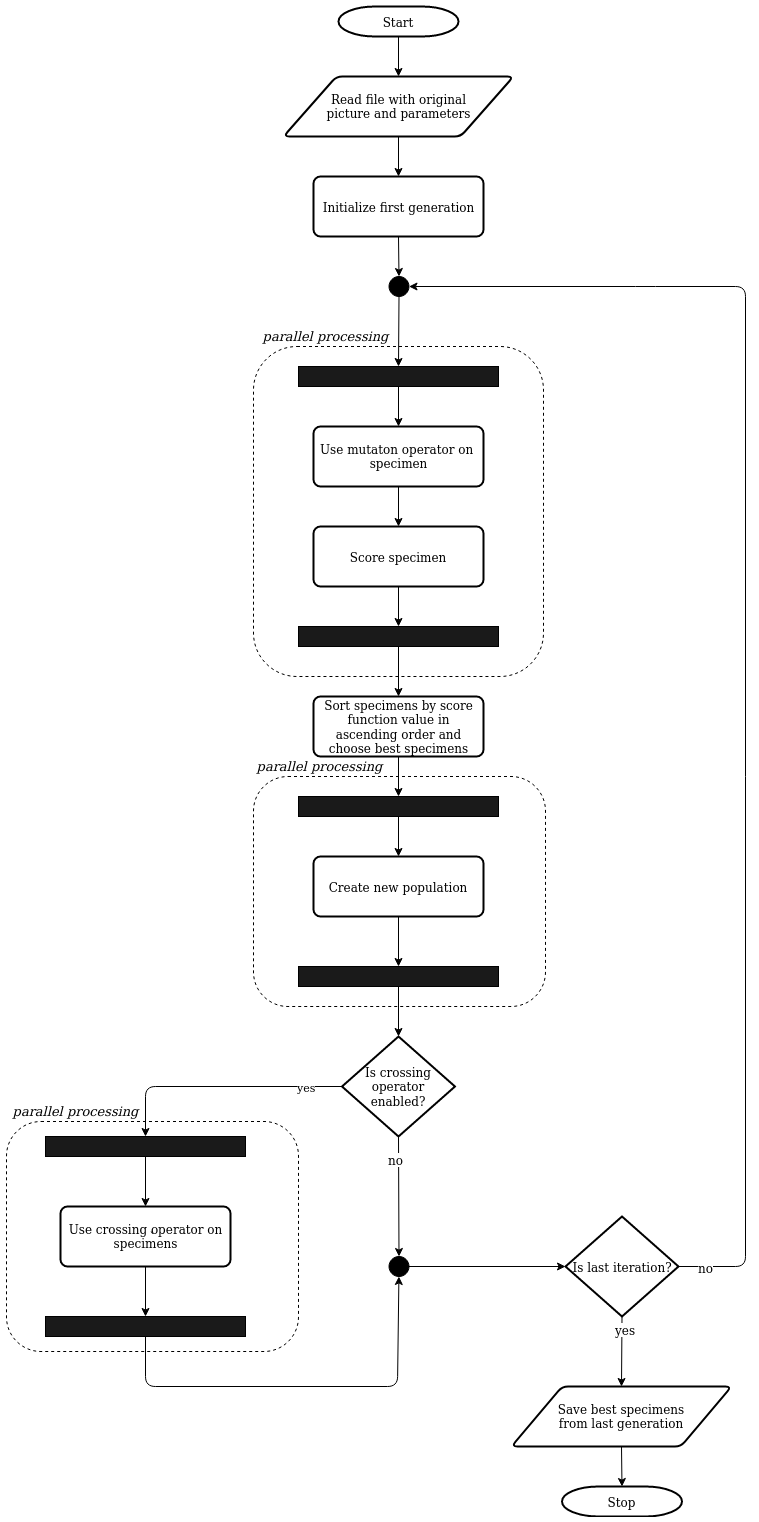
\includegraphics[scale=0.38]{images/other/thesis_flowchart.png}
    \caption{Diagram przepływu dla aplikacji. Program, po rozpoczęciu działania wczytuje odpowiednie pliki i parametry konfiguracyjne oraz inicjalizuje pierwsze pokolenie. Następnie stosowane są operator mutacji oraz funkcja oceny. Dalej tworzona jest nowa populacja i, jeżeli konfiguracja to przewiduje, stosowany jest operator krzyżowania. Program kończy działanie po określonej liczbie iteracji i zapisuje wyniki do odpowiednich plików po czym kończy działanie. Części algorytmu, które zostały urównoleglone zostały odpowiednio opisane na diagramie. Szczegółowy jego opis znajduje się w rozdziale \ref{sec:flowchart_desc}.}
    \label{fig:flowchart}
\end{figure}

\section{Komponenty aplikacji}
\label{sec:components_desc}
Prezentowana w pracy aplikacja składa się z różnych komponentów, gdzie każdy z nich spełnia określoną funkcjonalność niezbędną dla poprawnego działania aplikacji. W prezentowanej implementacji można wyróżnić następujące komponenty, które zostały przedstawione również na diagramie \ref{fig:components_chart}.

\subsection{Moduł konfiguracji}
\label{subsec:configuration_module}
Moduł odpowiedzialny za konfigurację algorytmu wczytuje parametry, które pozwalają na zdefiniowanie sposobu działania programu i przetrzymuje je w pamięci operacyjnej w taki sposób, aby były one dostępne dla pozostałych modułów aplikacji. 

\subsection{Moduł obsługi wejścia/wyjścia}
\label{subsec:io_module}
Moduł jest odpowiedzialny za wczytywanie plików (obraz, który ma zostać zreplikowany) oraz zapisanie rozwiązań wygenerowanych przez program po ostatniej iteracji algorytmu. Moduł obsługuje i wyświetla błędy związane z obsługą plików.

\subsection{Moduł genetyki}
\label{subsec:genetics_module}
Moduł obsługuje i definiuje działanie operatorów genetycznych (mutacji i krzyżowania) oraz odpowiada za wyliczanie funkcji celu dla każdego osobnika. Moduł ten jest \textit{wymienny} i może zostać przedefiniowany przez użytkownika przy warunku spełniania zadanego przez autora interfejsu.

\subsection{Moduł funkcji pomocniczych}
\label{subsec:helpers_module}
Komponent zawierający funkcje pomocnicze służące, między innymi, do sortowania osobników względem podanej wartości (w tym przypadku - względem funkcji celu), wyliczania wartości koloru dla pikseli dla operator mutacji, wyliczania wartości pomocniczych dla modułu genetyki. Szczegółowa specyfikacja tego modułu jest zawarta w dokumentacji technicznej kodu.

\subsection{Moduł obsługi współbieżności}
\label{subsec:threading_module}
Moduł odpowiedzialny za obsługę zadań, które mogą zostać obsłużone współbieżnie. Zostały one wyszczególnione na diagramie \ref{fig:flowchart}. Jego zadaniem jest rozdzielenie zadań pomiędzy poszczególne wątki oraz synchronizacja momentu ich zakończenia.

\begin{figure}
    \centering
    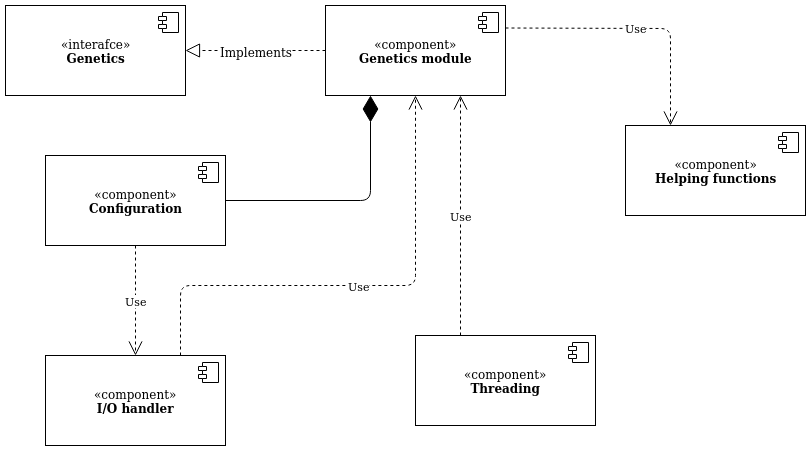
\includegraphics[scale=0.5]{images/other/components.png}
    \caption{Diagram komponentów aplikacji. Każdy z widocznych na grafice komponentów spełnia odpowiednią funkcjonalność, gdzie każdy z nich został krótko opisany w odpowiednim podrozdziale: interfejs \textit{Genetics} oraz komponent \textit{Genetics module} odpowiedzialne za logikę genetyki algorytmu opisane są w podrozdziale \ref{subsec:genetics_module}; \textit{Helping funcions} zawierajacy metody pomocnicze dla modułu genetyki opisany jest w podrozdziale \ref{subsec:helpers_module}; \textit{Configuration} odpowiedzialny za przechowywanie zdefiniowanej przez użytkownika konfiguracji algorytmu opisany jest w podrozdziale \ref{subsec:configuration_module}; \textit{Threading} odpowiedzialny za obsługę współbieżności w aplikacji opisany jest w sekcji \ref{subsec:threading_module}; moduł \textit{I/O handler} odpowiedzialny za obsługę wczytywanych i zapisywanych plików opisany jest w podrozdziale \ref{subsec:io_module}.
    }
    \label{fig:components_chart}
\end{figure}

	\cleardoublepage
	
	\chapter{Opis wykorzystywanych narzędzi}
\thispagestyle{chapterBeginStyle}

W tym rozdziale opisane zostaną wykorzystane narzędzia. Algorytm genetyczny, służący do replikacji obrazów, zostanie zaimplementowany w języku Go z wykorzystaniem wspieranej przez ten język współbieżności, a do analizy otrzymanych wyników zostanie wykorzystana biblioteka OpenCV oraz język Python.
	\cleardoublepage
	
	\chapter{Instrukcja użytkownika}
\thispagestyle{chapterBeginStyle}
\label{rozdzial4}

\section{Wymagania systemowe}

Program był testowany na systemach operacyjnych \texttt{Ubuntu 19.10 Eoan Ermine} oraz \texttt{macOS 10.15 Catalina} oraz przy użyciu języka \texttt{Go} w wersji \texttt{1.13}. Zaleca się uruchamianie programu na systemach \textit{unix-like} (np. \texttt{macOs}, \texttt{Ubuntu}, \texttt{Debian}, \texttt{ArchLinux}) oraz przy użyciu kompilatora \texttt{Go} co najmniej w wersji \texttt{1.11} ze względu na konieczność obsługi \texttt{Go modules}. Oprogramowanie nie zostało przetestowane na systemie operacyjnym \texttt{Windows} i nie jest gwarantowane jego działanie na tymże. 

\section{Parametry programu}
Tak jak opisano w rozdziałach poświęconych strukturze oraz implementacji algorytmu, program przyjmuje na wejściu zbiór argumentów pozwalających na konfigurację zachowania algorytmu. Poniżej zostanie przedstawiony sposób ich definiowania oraz uruchamiania programu. 

\subsection{Wywołanie konsolowe}
W przypadku, gdy program jest uruchamiany poprzez konsolę systemową parametry zostają zdefiniowane przez następujące flagi wywołania:
\begin{itemize}
    \item \texttt{-best} - flaga określa liczbę najlepszych osobników, które zostaną wybrane do tworzenia każdej kolejnej populacji oraz zapisane w ostatniej iteracji algorytmu, jako pliki wynikowe. Flaga ta powinna być liczbą typu \texttt{uint} (wartość domyślna: \texttt{10}).
    \item \texttt{-generation-size} - flaga określa rozmiar pojedynczego pokolenia w jednej iteracji algorytmu. Przyjmuje wartość typu \texttt{uint} (wartość domyślna: \texttt{200}).
    \item \texttt{-generations} - flaga określająca maksymalną liczbę iteracji algorytmu. Przyjmuje wartość typu \texttt{uint} (wartość domyślna: \texttt{1000}).
    \item \texttt{-gray-scale} - flaga określająca, czy algorytm powinien działać na obrazach w skali szarości. Flaga przyjmuje wartość typu \texttt{bool} (wartość domyślna: \texttt{false}).
    \item \texttt{-image-dir} - ścieżka do oryginalnego obrazu, który ma zostać zreplikowany przez algorytm. Flaga przyjmuje wartość typu \texttt{string}. Parametr ten jest wymagany, aby uruchomić program.
    \item \texttt{-mutation-chance} - flaga określająca prawdopodobieństwo wystąpienia mutacji. Flaga przyjmuje wartość typu \texttt{float} (wartość domyślna: \texttt{0.2}).
    \item \texttt{-with-crossing} - flaga określająca, czy powinien zostać zastosowany operator krzyżowania. Flaga przyjmuje wartość typu \texttt{bool} (wartość domyślna: \texttt{false}).
    \item \texttt{-from-file} - flaga przyjmuje ścieżkę do pliku konfiguracyjnego. Jeżeli została ona ustawiona, program ignoruje pozostałe flagi, jeśli są, i czyta parametry ze wskazanego pliku. Flaga przyjmuje wartość typu \texttt{string}.
    \item \texttt{-help} - jeżeli flaga jest ustawiona to zostają wyświetlone informacje na temat dostępnych parametrów wywołania, sposobu ich użycia oraz domyślnych wartości.
\end{itemize}

Program może zostać skompilowany za pomocą polecenia \texttt{go build main.go}, a następnie uruchomiony \texttt{./main}, lub bezpośrednio skompilowany i uruchomiony za pomocą polecenia \texttt{go run main.go}. Po zakończeniu działania programu można dokonać czyszczenia plików wygenerowanych przez kompilator za pomocą polecenia \texttt{go clean}. Wszystkie polecenia należy wywołać w głównym katalogu zawierającym plik \texttt{main.go}. 

\subsubsection{Przykładowe wywołania}
\begin{verbatim}
    #!/bin/bash
    go build main.go
    ./main -image-dir ./images/image_in_gray_scale.png \
            -best 5 \
            -generation-size 50 \
            -generations 5000 \
            -gray-scale \
            -mutation-chance 0.6 \
            -with-crossing 
    go clean
    
    go run main.go -image-dir ./images/image_in_rgba_scale.png
\end{verbatim}

\subsection{Plik konfiguracyjny}
Alternatywnym rozwiązaniem jest przekazanie parametrów wywołania przez plik konfiguracyjny. Aby to zrobić, należy użyć flagi \texttt{-from-file} i podać ścieżkę do tego pliku. Konfiguracja powinna zostać zapisana w formacie \texttt{JSON}. Dostępne są następujące atrybuty, które mogą zostać przekazane poprzez plik konfiguracyjny.

\subsubsection{Przykładowy plik konfiguracyjny}
\begin{verbatim}
    {
        "NumOfIterations": 2000,
        "SizeOfGeneration": 50,
        "PathToImage": "./images/example_image.jpg",
        "NumOfBest": 4,
        "MutationChance": 0.8,
        "GrayScale": false,
        "WithCrossing": true
    }
\end{verbatim}

\subsubsection{Przykładowe uruchomienie programu z plikiem konfiguracyjnym}
\begin{verbatim}
    #!/bin/bash
    
    go run main.go -from-file ./config.json
\end{verbatim}

Każdy parametr ma swój odpowiednik w opisanych w poprzedniej części rozdziału fladze wywołania programu.
\begin{itemize}
    \item \texttt{NumOfBest} - parametr określa liczbę najlepszych osobników, które zostaną wybrane do tworzenia każdej kolejnej populacji oraz zapisane w ostatniej iteracji algorytmu, jako pliki wynikowe. Parametr ten powinien być liczbą typu \texttt{uint} (wartość domyślna: \texttt{10}).
    \item \texttt{SizeOfGeneration} - parametr określa rozmiar pojedynczego pokolenia w jednej iteracji algorytmu. Przyjmuje wartość typu \texttt{uint} (wartość domyślna: \texttt{200}).
    \item \texttt{NumOfIterations} - parametr określający maksymalną liczbę iteracji algorytmu. Przyjmuje wartość typu \texttt{uint} (wartość domyślna: \texttt{1000}).
    \item \texttt{GrayScale} - parametr określający, czy algorytm powinien działać na obrazach w skali szarości. Flaga przyjmuje wartość typu \texttt{bool} (wartość domyślna: \texttt{false}).
    \item \texttt{PathToImage} - ścieżka do oryginalnego obrazu, który ma zostać zreplikowany przez algorytm. Parametr przyjmuje wartość typu \texttt{string}.
    \item \texttt{MutationChance} - parametr określający prawdopodobieństwo wystąpienia mutacji. Przyjmuje on wartość typu \texttt{float} (wartość domyślna: \texttt{0.2}).
    \item \texttt{WithCrossing} - Parametr określający, czy powinien zostać zastosowany operator krzyżowania. Przyjmuje wartość typu \texttt{bool} (wartość domyślna: \texttt{false}).
\end{itemize}

W przypadku, gdy któryś z parametrów nie zostanie wyspecyfikowany w pliku, przyjmie on wartość domyślną. Ponownie, jak w przypadku użycia flag wywołania, koniecznym jest zdefiniowanie parametru \texttt{PathToImage} (odpowiednik \texttt{-image-dir}).

\section{Docker}
Program może zostać uruchomiony z użyciem oprogramowania \texttt{Docker}. W tym celu zaleca się instalację pakietu \texttt{Docker} w ostatniej dostępnej wersji (testowano na wersji \texttt{19.03.5}). W celu uruchomienia programu należy użyć komendy \texttt{docker-compose up} w folderze zawierającym kod źródłowy programu. W przypadku uruchamiania programu w ten sposób, konfiguracja programu musi zostać podana poprzez plik konfiguracyjny \texttt{config.json} znajdujący się w głównym katalogu z kodem. W przypadku potrzeby modyfikacji ustawień Dockera (w tym - ścieżki dostępowej do pliku konfiguracyjnego), należy dokonać zmian w pliku \texttt{docker-compose.yaml} zgodnie z dokumentacją tego oprogramowania [cf. \cite{DockerDocs}].

\section{Modyfikacja modułu genetyki algorytmu}
\label{sec:genetics_interface_modifications}

Moduł odpowiedzialny za genetykę algorytmu został zaimplementowany jako interfejs w języku \texttt{Go} i jest on \textit{wymienny}, to jest możliwe jest wykonanie własnej jego implementacji pod warunkiem spełniania określonego interfejsu przedstawionego w \ref{lst:genetics_interface}.
\begin{lstlisting}[caption={Interfejs modułu genetyki}, captionpos=b, label={lst:genetics_interface}]
type Genetics interface {
	Mutate()
	Fitness(originalImage image.Image)
	Cross(spec image.RGBA)
}
\end{lstlisting}
W celu własnego zdefiniowania należy zaimplementować metody spełniające interfejs zaprezentowany na \ref{lst:genetics_interface} mając na uwadze, że metoda \texttt{Mutate()} definiuje sposób dokonywania mutacji; metoda \texttt{Fitness(originalImage image.Image)} definiuje funkcję oceny i jako parametr przyjmuje referencję do obrazu oryginalnego; metoda
\texttt{Cross(spec image.RGBA)} definiuje sposób krzyżowania osobników i jako parametr przyjmuje referencję do osobnika, z którym dany osobnik ma być krzyżowany. Należy mieć na uwadze, że są to struktury z \textit{dowiązanymi} metodami (ang. \textit{function-like objects}) i mogą się odwoływać do pól struktury, na której operują. Przykład został zaprezentowany takiej struktury został zaprezentowany na \ref{lst:function_like_object}.

\begin{lstlisting}[caption={Przykład \textit{function-like object}}, captionpos=b, label={lst:function_like_object}]
type dummyStruct struct {
    dummyProperty string
} 

func (ds *dummyStruct) dummyMethod() {

}
\end{lstlisting}

W celu użycia własnego przygotowanego modułu należy podmienić plik \texttt{module.go} znajdujący się w katalogu \texttt{/src/genetics}, w którym zaimplementowana jest domyślna genetyka.
	\cleardoublepage
	
	\chapter{Analiza wyników}
\thispagestyle{chapterBeginStyle}
\label{rozdzial5}

W ramach pracy dokonano szeregu testów przygotowanej implementacji algorytmu replikacji obrazów. Autor skupił się na tym, aby uzyskać jak najlepsze wyniki, stąd zdecydował się jedynie do metody tworzenia kolejnego pokolenia jedynie z najlepszych osobników z bieżącej iteracji, z jednoczesną możliwością zbadania pewnych parametrów, które pozwolą na stworzenie pewnego schematu działania algorytmów oraz analizę jakości ich działania. Jako osobniki \textit{najlepsze} należy rozumieć te, które są najbardziej \textit{podobne} do obrazu oryginalnego pod względem wartości funkcji celu (funkcja celu jest dla nich jak najmniejsza). Drugorzędnym kryterium oceny była w tym przypadku ocena wizualna. Obranie takiego kryterium wyboru osobników do utworzenia każdego kolejnego pokolenia wynika z faktu, że algorytm do oceny poszczególnych rozwiązań używa regularnej funkcji celu, która posiada lokalne optima z niewielką amplitudą.

W tym rozdziale zostaną przedstawione i omówione przeprowadzone testy. Autor skupił się tutaj na przedstawieniu postawionych hipotez odnośnie wpływu poszczególnych parametrów na jakość uzyskiwanych rozwiązań, analizie i prezentacji uzyskanych wyników oraz wyciągniętych na ich podstawie wniosków odnośnie zależności jakości uzyskiwanych obrazów a danym parametrem. 

Większość prezentowanych w tym rozdziale przykładów będzie opierać się na obrazie \textit{Mona Lisa} autorstwa Leonarda da Vinci, a dokładniej - na jego zdjęciu. Autor zdecydował się na wykorzystanie tego dzieła malarskiego ze względu na fakt, że jest to jeden z popularniejszych obrazów, które są wykorzystywane do prezentowania rezultatów w podobnych implementacjach dostępnych w sieci. Ma to na celu umożliwienie porównania czytelnikowi możliwości zaimplementowanego algorytmu z innymi dostępnymi rozwiązaniami wykorzystującymi podobne lub te same techniki.

\section{Rozmiar populacji}
\label{sec:population}
Dla problemu wpływu rozmiaru pojedynczej populacji na jakość otrzymywanych wyników autor pracy postawił następującą hipotezę:

\begin{hypothesis}
Liczba osobników w każdym pokoleniu wpływa na jakość ostatecznego rozwiązania zwracanego przez algorytm. Wraz ze wzrostem liczby osobników rośnie różnorodność osobników z unikalnym materiałem genetycznym, a przez co wzrasta również prawdopodobieństwo uzyskania osobników lepiej ocenianych przez funkcję celu.
\end{hypothesis}

W celu sprawdzenia powyższej hipotezy wykonano testy pozwalające zbadać wpływ parametru odpowiadającego za rozmiar pojedynczej populacji. Przeprowadzono testy na zdjęciu obrazu \textit{Mona Lisa} autorstwa Leonarda da Vinci zapisany jako plik \texttt{PNG} w skali RGBA - rysunek \ref{fig:mona_rgba}. Zbadano jak wpływa liczebność pojedynczego pokolenia dla określonej liczby iteracji na jakość uzyskanego rozwiązania.

\begin{figure}[!htb]
    \centering
    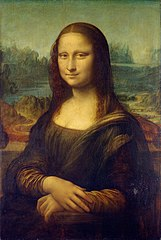
\includegraphics{images/mona/mona.jpg}
    \caption{
        Replikowany obraz \textit{Mona Lisa} w skali \texttt{RGBA}
        \textit{(Źródło: \cite{MonaLisa}})
    }
    \label{fig:mona_rgba}
\end{figure}

\subsection{Obserwacje}
Na rysunku \ref{fig:generations_1} przedstawiono jakość najlepszych rozwiązań (najlepiej ocenionych przez funkcję celu) po 1000 pokoleń odpowiednio dla 10, 50, 100 oraz 300 osobników w jednym pokoleniu. Zgodnie z tym, jak to opisano na początku niniejszego rozdziału, wybrano metodykę, w której każde kolejne pokolenie tworzone jest jedynie z \textit{pewnej} (określonej przez parametr podany przez użytkownika) liczby osobników, które zostały ocenione najwyżej przez funkcję celu. W tym, konkretnym przypadku dla takich osobników funkcja celu będzie miała wartość najmniejszą, co świadczy o fakcie, że odległość pomiędzy tymi rozwiązaniami a obrazem oryginalnym jest najmniejsza. Widoczna jest jedna znacząca różnica pomiędzy poszczególnymi prezentowanymi osobnikami pod względem wizualny. Na osobniku, który pochodził z testu, gdzie na pokolenie przypadało 300 osobników, można zauważyć wyraźny zarys postaci oraz elementów tła. Podobnie jest dla osobnika pochodzącego z testu, gdzie na pokolenie przypadało 100 osobników. W przypadku, gdy pokolenia miały liczność odpowiednio 50 i 10 osobników zauważenie konturów tła i postaci jest już praktycznie niemożliwe. Obraz z testu, w którym kolejne populacje liczyły po 10 obrazów, po 1000 iteracji obraz, pod względem wizualnym, w żaden sposób nie przypomina obrazu, do którego replikacji algorytm dąży. 

\begin{figure}[!htb]
    \centering
    \begin{subfigure}[b]{0.3\textwidth}
        \centering
         
\includegraphics[width=\textwidth]{images/mona/10000_10_2/img_0_it_1000_best.png}
         \caption{10 osobników/pokolenie}
    \end{subfigure}
    \begin{subfigure}[b]{0.3\textwidth}
        \centering
         
\includegraphics[width=\textwidth]{images/mona/10000_50_2/img_0_it_1000_best.png}
         \caption{50 osobników/pokolenie}
    \end{subfigure}
     \begin{subfigure}[b]{0.3\textwidth}
        \centering
         
\includegraphics[width=\textwidth]{images/mona/10000_100_2/img_0_it_1000_best.png}
         \caption{100 osobników/pokolenie}
    \end{subfigure}
     \begin{subfigure}[b]{0.3\textwidth}
        \centering
         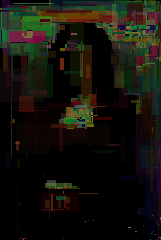
\includegraphics[width=\textwidth]{images/mona/10000_300_2/img_0_it_1000_best.png}
         \caption{300 osobników/pokolenie}
    \end{subfigure}
    \caption{Wyniki replikacji dla różnych liczności pokolenia dla 1000 iteracji algorytmu}
    \label{fig:generations_1}
\end{figure}


\subsection{Wnioski}
Zauważalna jest wyraźna wizualna różnica pomiędzy poszczególnymi zaprezentowanymi wynikami, dla różnych wartości parametru odpowiadającego za liczebność pokolenia, a obrazem zreplikowanym \ref{fig:mona_rgba}. Na podstawie prezentowanych wyników można stwierdzić, że liczebność pojedynczego pokolenia ma zdecydowany wpływ na jakość otrzymywanych rozwiązań - zarówno pod względem wizualnym, jak i względem wartości zwracanych przez funkcję celu. Potwierdza to postawione w hipotezie przypuszczenie, że wzrost liczby osobników powoduje, że różnorodność \textit{materiału genetycznego} jest większa (większa liczba osobników implikuje większą unikalność gwarantowaną przez operator mutacji). W takim przypadku algorytm wybiera osobniki do następnej iteracji z większej puli rozwiązań. Istnieje zatem większe prawdopodobieństwo zajścia mutacji (wzmocnionej potem przez operator krzyżowania) takiej, że osobnik z mutacją znacząco przybliży się, względem wartości funkcji oceny, do obrazu oryginalnego.

\section{Liczba pokoleń}
\begin{hypothesis}
Liczba pokoleń (iteracji) algorytmu wpływa na jakoś ostatecznego rozwiązania zwracanego przez algorytm. Wraz ze wzrostem liczby iteracji algorytmu zachodzi więcej zmian w materiale genetycznym osobników, przez co rośnie prawdopodobieństwo otrzymania rozwiązania bardziej zbliżonego, względem wartości funkcji celu, do obrazu replikowanego.
\end{hypothesis}

\subsection{Obserwacje}
W celu zbadania tego parametru ponownie zreplikowano obraz \ref{fig:mona_rgba}. Wyniki zaprezentowano na grafice \ref{fig:iterations_1}. Widoczna jest znacząca różnica pomiędzy rozwiązaniem uzyskanym po 100 iteracjach algorytmu, a rozwiązaniem uzyskanym w ostatniej, 10000., iteracji. Jednocześnie można zauważyć, że pomiędzy obrazem uzyskanym w 5000. iteracji, a osobnikiem z 10000. iteracji nie da się zauważyć, pod względem wizualnym, już wielu różnic.

\begin{figure}[!htb]
    \centering
    \begin{subfigure}[b]{0.3\textwidth}
        \centering
         
\includegraphics[width=\textwidth]{images/mona/10000_300_2/img_0_it_100_best.png}
         \caption{100 iteracji}
    \end{subfigure}
    \begin{subfigure}[b]{0.3\textwidth}
        \centering
         
\includegraphics[width=\textwidth]{images/mona/10000_300_2/img_0_it_500_best.png}
         \caption{500 iteracji}
    \end{subfigure}
    \begin{subfigure}[b]{0.3\textwidth}
        \centering
         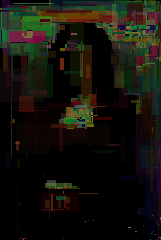
\includegraphics[width=\textwidth]{images/mona/10000_300_2/img_0_it_1000_best.png}
         \caption{1000 iteracji}
    \end{subfigure}
    \begin{subfigure}[b]{0.3\textwidth}
        \centering
         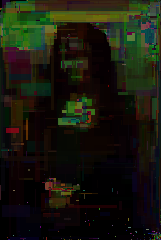
\includegraphics[width=\textwidth]{images/mona/10000_300_2/img_0_it_5000_best.png}
         \caption{5000 iteracji}
    \end{subfigure}
    \begin{subfigure}[b]{0.3\textwidth}
        \centering
         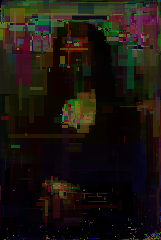
\includegraphics[width=\textwidth]{images/mona/10000_300_2/img_0_it_10000_best.png}
         \caption{10000 iteracji}
    \end{subfigure}
    \caption{Wyniki replikacji odpowiednio dla 100, 500, 1000, 5000 oraz 10000 iteracji algorytmu z liczebnością każdego pokolenia - 300 osobników}
    \label{fig:iterations_1}
\end{figure}

\subsection{Wnioski}
Na podstawie zaprezentowanych wyników można stwierdzić, że liczba iteracji algorytmu ma znaczący wpływ na jakość zwracanych rozwiązań. Wraz z każdą kolejną iteracją algorytmu widać, że z każdą kolejną iteracją zauważalna jest większa liczba podobieństw między konkretnym rozwiązaniem a obrazem replikowanym. Wynika to z faktu, że z każdą kolejną iteracją, genotyp poszczególnych osobników jest wzbogacany przez stosowane operatory genetyczne. Podobnie, jak ma to miejsce w przypadku opisanego w podrozdziale \ref{sec:population}, w tym przypadku również rośnie prawdopodobieństwo uzyskania obrazu bardziej zbliżonego do oryginału. Czynnikiem decydującym w tym przypadku jest nie ilość osobników w pojedynczym pokoleniu, ale liczba iteracji. Podobnie, jak ma to miejsce w naturalnym procesie ewolucji, z każdym kolejnym pokoleniem w osobnikach zachodzą zmiany genetyczne. Dysponując dużą pulą osobników można uzyskać wiele różnych zmian w genotypie, a powtarzając tę operację określoną liczbę razy, uzyskać wynik bardziej zbliżony do oryginalnego. Należy stwierdzić zatem, że zarówno parametr odpowiadający za liczbę pokoleń w algorytmie, jak i parametr odpowiedzialny za określenie mnogości każdego pokolenia, są ze sobą w ścisły sposób powiązane. 

Kolejnym wnioskiem, wynikającym z obserwacji dotyczącej niewielkich zmian pomiędzy 5000. a 10000. pokoleniem, jest to, że prezentowany algorytm replikacji może utknąć w lokalnym optimum. Oznacza to, że uzyskiwane odchylenia funkcji celu będą się mieścić w pewnym wąskim przedziale i nie będą się już znacząco powiększać. Od strony wizualnej, każde kolejne zmiany będą już praktycznie niezauważalne.

\section{Skala barw}
\begin{hypothesis}
Zastosowana w obrazie oryginalnym skala barw (rozważane są skala RGBA oraz skala szarości) ma pływ na jakość uzyskanych rozwiązań. Dla skali szarości (obrazy jednokanałowe) algorytm jest w stanie odtworzyć więcej szczegółów obrazu replikowanego, niż w przypadku zastosowania skali RGBA (obrazy czterokanałowe).
\end{hypothesis}
\begin{figure}[!htb]
    \centering
    \includegraphics[scale=4.0]{images/mona/mona_bw.jpg}
    \caption{Replikowany obraz \textit{Mona Lisa} w skali szarości (\textit{Źródło}: \cite{MonaLisa})}
    \label{fig:monra_bw}
\end{figure}
\subsection{Obserwacje}
W celu zaobserwowania różnic dla różnych skali barw dokonano replikacji obrazów \ref{fig:mona_rgba} oraz \ref{fig:monra_bw} dla takich samych parametrów wejściowych. Wyniki (dla 10000. pokolenia) zaprezentowano na grafice \ref{fig:scale_1}. Pod względem wizualnym, zauważalnym jest, że dla obrazu, który replikowany był w odcieniach szarości, widoczna jest większa liczba szczegółów, niż dla obrazu prezentowanego w skali RGBA. Porównywanie wartości funkcji celu, ze względu na dwie odmienne skale barw, zostanie tutaj pominięte.

\begin{figure}[!htb]
    \centering
    \begin{subfigure}[b]{0.3\textwidth}
        \centering
        \label{fig:scale_1_rgba}
         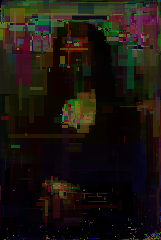
\includegraphics[width=\textwidth]{images/mona/10000_300_2/img_0_it_10000_best.png}
         \caption{Skala RGBA}
    \end{subfigure}
    \begin{subfigure}[b]{0.3\textwidth}
        \centering
        \label{fig:scale_1_bw}
         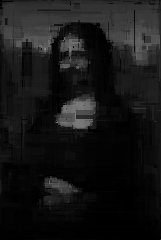
\includegraphics[width=\textwidth]{images/mona/10000_300_2/img_0_best.png}
         \caption{Skala szarości}
    \end{subfigure}
    \caption{Porównanie wyników replikacji dla skali szarości i RGBA \textit{ (10000 pokoleń, 300 osobników w pokoleniu}}
    \label{fig:scale_1}
\end{figure}

\subsection{Wnioski}
Wyniki replikacji w skali szarości pozwoliły na uzyskanie większej ilości szczegółów względem pierwowzoru, ze względu na fakt, że rozważany jest wówczas tylko jeden kanał i, w konsekwencji, podczas mutacji losowana jest tylko pojedyncza wartość. W przypadku skali RGBA takie wartości muszą być wylosowane cztery co jednocześnie zwiększa liczbę możliwych konfiguracji wartości dla wszystkich kanałów, przez co prawdopodobieństwa \textit{trafienia} w wartość koloru, który byłby jak najmniej oddalony od koloru danego piksela na obrazie oryginalnym maleje.

\section{Prawdopodobieństwo mutacji}
Kolejnym badanym parametrem, mającym wpływ na jakość uzyskanych rozwiązań był parametr odpowiadający za prawdopodobieństwo wystąpienia na danym osobniku mutacji. Ponownie zbadano wpływ parametru na jakość uzyskiwanych rozwiązań dla obrazu \ref{fig:mona_rgba}.

\begin{hypothesis}
Większa wartość parametru $p_{m}$ określającego prawdopodobieństwo wystąpienia mutacji wpływa na szybkość zbiegania algorytmu.
\end{hypothesis}

\subsection{Obserwacje}
Zbadano jakość uzyskiwanych rozwiązań dla parametru prawdopodobieństwa wystąpienia mutacji $p_{m} \in \lbrace 0.2, 0.4, 0.6, 0.8 \rbrace$. Wyniki przeprowadzonych testów zaprezentowano na grafice \ref{fig:mutation_1}. W tabeli \ref{tab:mutation_scores} przedstawiono wartości funkcji celu dla poszczególnych parametrów. Widoczne jest malenie wartości funkcji celu $f_{c}$ wraz ze wzrostem wartości parametru $p_{m}$. Pod względem wizualnym również daje się zauważyć, że na obrazach, gdzie prawdopodobieństwo wystąpienia mutacji było większe, odwzorowanie jest bardziej szczegółowe i na obrazach tych wyraźniej widoczna jest sylwetka postaci z obrazu będącego ich pierwowzorem.

\begin{table}[h]
    \centering
    \begin{tabular}{|c|c|}
        \hline
        $p_{m}$ & $f_{c}$  \\
        \hline
        $0.2$ & $496634177696466.0$ \\
        \hline
        $0.4$ & $496634145298532.0$ \\
        \hline
        $0.6$ & $496634099405528.0$ \\
        \hline
        $0.8$ & $496633985597704.0$ \\
        \hline
    \end{tabular}
    \caption{Wartości funkcji celu dla różnych wartości parametru $p_{m}$ określającego prawdopodobieństwo wystąpienia mutacji. Wyniki dla obrazów prezentuje rysunek \ref{fig:mutation_1}.}
    \label{tab:mutation_scores}
\end{table}

\begin{figure}[!htb]
    \centering
    \begin{subfigure}[b]{0.3\textwidth}
        \centering
        \label{fig:mutation_0_2}
         
\includegraphics[width=\textwidth]{images/mona/1000_300_2/mutation/0_2.png}
         \caption{$p_{m} = 0.2$}
    \end{subfigure}
    \begin{subfigure}[b]{0.3\textwidth}
        \centering
        \label{fig:mutation_0_4}
         
\includegraphics[width=\textwidth]{images/mona/1000_300_2/mutation/0_4.png}
         \caption{$p_{m} = 0.4$}
    \end{subfigure}
    \begin{subfigure}[b]{0.3\textwidth}
        \centering
        \label{fig:mutation_0_6}
         
\includegraphics[width=\textwidth]{images/mona/1000_300_2/mutation/0_6.png}
         \caption{$p_{m} = 0.6$}
    \end{subfigure}
    \begin{subfigure}[b]{0.3\textwidth}
        \centering
        \label{fig:mutation_0_8}
         
\includegraphics[width=\textwidth]{images/mona/1000_300_2/mutation/0_8.png}
         \caption{$p_{m} = 0.8$}
    \end{subfigure}
    \caption{Porównanie wyników replikacji dla różnych wartości parametru $p_{m}$ określającego prawdopodobieństwo mutacji \textit{1000 iteracji, 300 osobników w pokoleniu}}
    \label{fig:mutation_1}
\end{figure}

\subsection{Wnioski}
Na podstawie przedstawionych obserwacji łatwo zauważyć, że większa wartość parametru określającego prawdopodobieństwo wystąpienia mutacji w danym osobniku pozytywnie wpływa na jakość uzyskiwanych rozwiązań. Im większe prawdopodobieństwo mutacji, tym większa szansa, że do genotypu danego osobnika zostanie wprowadzona \textit{pozytywna} zmiana. Przez \textit{pozytywną} zmianę rozumie się taką, która sprawie, że odległość pomiędzy wygenerowanym rozwiązaniem, a obrazem oryginalnym zmniejsza się w stosunku do stanu, zanim mutacja została wprowadzona. Należy też w tym miejscu zauważyć, że większa wartość parametru $p_{m}$ niekoniecznie musi gwarantować uzyskanie lepszych wyników. Może bowiem dojść do takiej sytuacji, że genotyp osobników będzie w taki sposób modyfikowany, że zmiany nie będą korzystne dla oczekiwanych rezultatów, to jest mogą zostać wprowadzone zmiany, które sprawią, że osobniki w kolejnym pokoleniu mogą zostać ocenione gorzej od osobników z pokolenia poprzedniego.

\section{Liczba osobników wybieranych do utworzenia populacji}
W następnej kolejności zbadano wpływ liczby osobników wybieranych jako najlepsze w danym pokoleniu do utworzenia kolejnej populacji na jakość uzyskiwanych rozwiązań. 

\begin{hypothesis}
Wzrost liczby najlepiej przez funkcję celu ocenianych osobników wybieranych do następnego pokolenia zmniejsza prawdopodobieństwo zbiegania algorytmu do optymalnego rozwiązania.
\end{hypothesis}

\subsection{Obserwacje}
W tym przypadku autor ponownie zbadał to zjawisko na podstawie replikacji obrazu \ref{fig:mona_rgba}. Wyniki zaprezentowano na grafice \ref{fig:num_of_best}. Bardzo wyraźnie widać, że wraz ze wzrostem liczby osobników wybieranych do tworzenia kolejnego pokolenia zarys sylwetki widocznej na obrazie kobiety zaczyna być co raz mniej dostrzegalny. Dla 200 wybieranych osobników, po 1000 iteracji algorytmu na obrazie widać jedynie losowy szum, który zupełnie nie przypomina pierwowzoru. 

\begin{figure}[!htb]
    \centering
    \begin{subfigure}[b]{0.3\textwidth}
        \centering
        \label{fig:num_of_best_2}
         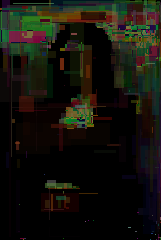
\includegraphics[width=\textwidth]{images/mona/num_of_best/2.png}
         \caption{2 osobniki}
    \end{subfigure}
    \begin{subfigure}[b]{0.3\textwidth}
        \centering
        \label{fig:num_of_best_10}
         
\includegraphics[width=\textwidth]{images/mona/num_of_best/10.png}
         \caption{10 osobników}
    \end{subfigure}
    \begin{subfigure}[b]{0.3\textwidth}
        \centering
        \label{fig:num_of_best_50}
         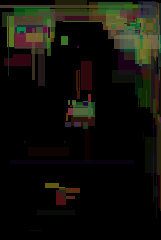
\includegraphics[width=\textwidth]{images/mona/num_of_best/50.png}
         \caption{50 osobników}
    \end{subfigure}
    \begin{subfigure}[b]{0.3\textwidth}
        \centering
        \label{fig:num_of_best_100}
         
\includegraphics[width=\textwidth]{images/mona/num_of_best/100.png}
         \caption{100 osobników}
    \end{subfigure}
    \begin{subfigure}[b]{0.3\textwidth}
        \centering
        \label{fig:num_of_best_200}
         
\includegraphics[width=\textwidth]{images/mona/num_of_best/200.png}
         \caption{200 osobników}
    \end{subfigure}
    \caption{Porównanie wyników replikacji dla różnej liczby osobników wykorzystanych do tworzenia nowego pokolenia \textit{(1000 pokoleń, 300 osobników w pokoleniu)}}
    \label{fig:num_of_best}
\end{figure}

\subsection{Wnioski}
Wraz ze wzrostem liczby osobników, z których jest tworzone kolejne pokolenie maleje czytelność uzyskiwanych wyników. Dla wartości parametru 2, 50 i 100 daje się jeszcze na obrazie rozróżnić sylwetkę kobiety z oryginalnego obrazu. W przypadku wartości 100 i 200 na obrazach widoczny jest jedynie losowy szum. Wynika to z faktu, że wraz ze wzrostem liczby wyselekcjonowanych osobników, do następnego pokolenia dostają się również osobniki gorzej ocenione przez funkcję celu. W konsekwencji tego wybór staje się bardziej losowy. Na podstawie obserwacji można stwierdzić, że im mniej osobników zostało wybranych do utworzenia nowej populacji, tym algorytm szybciej zbiega do oczekiwanego rozwiązania.

\section{Złożoność obrazu}
Ostatnim zbadanym czynnikiem, mogącym mieć wpływ na jakość uzyskiwanych wyników, a przez to - na szybkość zbiegania algorytmu, była złożoność replikowanego obrazu. 

\begin{hypothesis}
Wraz ze wzrostem liczby szczegółów na replikowanym obrazie maleje dokładność jego odwzorowania.
\end{hypothesis}

Postawioną powyżej hipotezę sprawdzono na kilku obrazach o różnym stopniu skomplikowania zaprezentowanych na grafice przedstawionych na rysunku \ref{fig:complexity_original}. Obraz \textbf{(a)} przedstawia zdjęcie twarzy wygenerowanej przez sztuczną inteligencję. Mimo sporej liczby szczegółów, twarz osoby obecnej na zdjęciu zajmuje sporą część zdjęcia przez to jest elementem zajmującym większość przestrzeni na obrazie. Ponadto obraz ten posiada jednokolorowe tło. Na \textbf{(b)} przedstawiona portret postaci w taki sposób, że jest ona widoczna do końca jej tułowia. Obraz zawiera sporo szczegółów w tle jak i na ubraniu, które ma na sobie sportretowana kobieta (zagięcia, cienie). Ostatni obraz \textbf{(c)}, zawiera wiele elementów o różnym stopniu jasności i skomplikowania.

\begin{figure}[!htb]
    \centering
    \begin{subfigure}[b]{0.3\textwidth}
        \centering
        \label{fig:complexity_ai}
         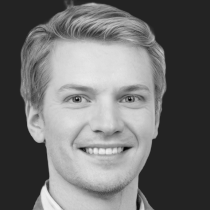
\includegraphics[width=\textwidth]{images/complexity/originals/ai2.png}
         \caption{Zdjęcie twarzy wygenerowane przez AI (\textit{Źródło}: \cite{AIFace})}
    \end{subfigure}
    \begin{subfigure}[b]{0.3\textwidth}
        \centering
        \label{fig:complexity_mona}
         \includegraphics[width=\textwidth]{images/complexity/originals/mona_bw.jpg}
         \caption{\textit{Mona Lisa}, Leonardo da Vinci (\textit{Źródło}: \cite{MonaLisa})}
    \end{subfigure}
    \begin{subfigure}[b]{0.8\textwidth}
        \centering
        \label{fig:complexity_guernica}
         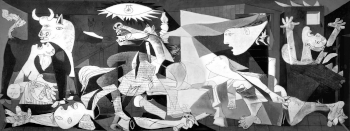
\includegraphics[width=\textwidth]{images/complexity/originals/gueranica_bw.png}
         \caption{\textit{Guernica}, Pablo Picasso (\textit{Źródło}: \cite{Guernica})}
    \end{subfigure}
    \caption{Obrazy o różnej złożoności pod względem liczby obecnych na nich szczegółów}
    \label{fig:complexity_original}
\end{figure}

\subsection{Obserwacje}
Wyniki replikacji obrazów przedstawia grafika \ref{fig:complexity_rep}. Widać, że algorytm poradził sobie najlepiej z obrazem \textbf{(a)}, na którym widoczna była sama twarz, a najgorzej z tymi, które wymagały odwzorowania wielu elementów o różnych rozmiarach. W przypadku dwóch pozostałych obrazów widać jedynie zarysy postaci. O ile w przypadku zreplikowanego obrazu \textbf{(b)} obserwator jest w stanie domyślać się, że jest to portret kobiety, o tyle w przypadku \textbf{(c)} ciężko stwierdzić co dokładnie zostało na obrazie przedstawione.

\begin{figure}[!htb]
    \centering
    \begin{subfigure}[b]{0.3\textwidth}
        \centering
        \label{fig:complexity_ai_rep}
         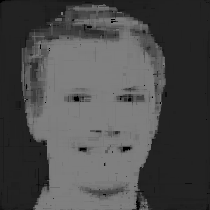
\includegraphics[width=\textwidth]{images/complexity/ai.png}
         \caption{Zdjęcie twarzy wygenerowane przez AI}
    \end{subfigure}
    \begin{subfigure}[b]{0.3\textwidth}
        \centering
        \label{fig:complexity_mona_rep}
         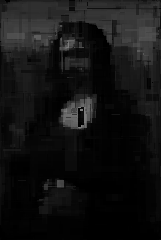
\includegraphics[width=\textwidth]{images/complexity/mona.png}
         \caption{\textit{Mona Lisa}, Leonardo da Vinci}
    \end{subfigure}
    \begin{subfigure}[b]{0.8\textwidth}
        \centering
        \label{fig:complexity_guernica_rep}
         
\includegraphics[width=\textwidth]{images/complexity/guernica.png}
         \caption{\textit{Guernica}, Pablo Picasso}
    \end{subfigure}
    \caption{Wyniki replikacji obrazów przedstawionych na \ref{fig:complexity_original} \textit{(10000 pokoleń, 300 osobników w pokoleniu)}}
    \label{fig:complexity_rep}
\end{figure}

\subsection{Wnioski}
Na podstawie przedstawionych obserwacji można wyciągnąć wnioski, że liczba szczegółów ma znaczący wpływ na szczegółowość odwzorowania obrazu. Przy okazji badania wpływu szczegółowości obrazu na jakość rozwiązania, warto zauważyć, że jest to również poniekąd związane z rozdzielczością obrazu. Im większy obraz, tym więcej szczegółów jest na nim widocznych.

\section{Czas działania programu}
Autor zbadał również zależność czasu działania algorytmu od dwóch najbardziej istotnych parametrów jakimi są liczba iteracji oraz rozmiar pojedynczego pokolenia. Wyniki zaprezentowano w tabelach \ref{tab:times_it} oraz \ref{tab:times_gen} (Testy przeprowadzono na systemie \texttt{macOS 10.15 Catalina} i sześciordzeniowym procesorze (16 wątków) Intel Core i7. Czas działania programu został zmierzony za pomocą konsolowego programu \texttt{time} dostępnego w systemach typu Unix-like).

\begin{table}[!htb]
    \centering
    \begin{tabular}{|c|c|c|}
        \hline
        $i$ & $N$ & $\mathrm{time}$ [$s$]  \\
        \hline
        $10000$ & $50$ & $294.52$ \\
        \hline
        $10000$ & $100$ & $540.48$ \\
        \hline
        $10000$ & $200$ & $1128.97$ \\
        \hline
        $10000$ & $300$ & $1731.64$ \\
        \hline
    \end{tabular}
    \caption{Czasy działania algorytmu (w sekundach) dla stałej liczby iteracji iteracji ($i$) oraz zmiennego rozmiaru pokolenia ($N$).}
    \label{tab:times_it}
\end{table}

\begin{table}[!htb]
    \centering
    \begin{tabular}{|c|c|c|}
        \hline
        $i$ & $N$ & $\mathrm{time}$ [$s$]  \\
        \hline
        $500$ & $200$ & $52.86$ \\
        \hline
        $1000$ & $200$ & $111.07$ \\
        \hline
        $5000$ & $200$ & $588.98$ \\
        \hline
        $10000$ & $200$ & $1731.64$ \\
        \hline
    \end{tabular}
    \caption{Czasy działania algorytmu (w sekundach) dla zmiennej liczby iteracji iteracji ($i$) oraz stałego rozmiaru pokolenia ($N$).}
    \label{tab:times_gen}
\end{table}

\subsection{Obserwacje}
Na podstawie przeprowadzonych obserwacji można zauważyć, że zarówno, gdy zmienia się rozmiar pokolenia przy stałej liczbie iteracji (tabela \ref{tab:times_it}), jak i w sytuacji, gdy zmianie ulega liczba iteracji, liczność pokolenia jest stała (tabela \ref{tab:times_gen}), czas działania programu rośnie wprost proporcjonalnie do zmieniającego się parametru.

\subsection{Wnioski}
W obu przypadkach wzrost czasu działania programy wynika z innej przyczyny. W sytuacji, gdy zmienia się jedynie rozmiar pokolenia, program wykonuje się dłużej, ponieważ w każdej iteracji potrzebuje więcej czasu na przetworzenie wszystkich osobników (zastosowanie operatorów mutacji i ocena). W przypadku, gdy stały jest rozmiar pokolenia, a zmienia się liczba iteracji fakt, że program działa dłużej wynika z tego, że chociaż w każdej iteracji przetworzenie wszystkich osobników w populacji zajmuje tyle samo czasu, ale wzrost jest spowodowany większą liczbą powtórzeń w programie.

\section{Parametry a ograniczenie czasowe}

Ostatnim elementem analizy jest zbadanie zależności pomiędzy liczbą iteracji i licznością pojedynczego pokolenia, w przypadku, gdy na algorytm zostało narzucone ograniczenie czasowe. Celem tego testu jest sprawdzenie, który parametr opłaca się zwiększyć (kosztem zmniejszenia wartości drugiego), aby uzyskać jak najlepsze wyniki. Autor przeprowadził testy na obrazie \ref{fig:monra_bw} dla różnych wartości liczby pokoleń algorytmu i rozmiaru populacji przy założeniu, że jest to zależność odwrotnie proporcjonalna (czas działania dla każdego był, w przybliżeniu, taki sam). Wyniki prezentuje grafika \ref{fig:dependence_rep}. Zbadane konfiguracje parametrów i czas działania programu dla każdej z nich przedstawiono w tabeli \ref{tab:dependence_times}. 

\begin{table}[!htb]
    \centering
    \begin{tabular}{|c|c|c|}
        \hline
        $i$ & $N$ & $\mathrm{time}$ [$s$]  \\
        \hline
        $10000$ & $50$ & $294.52$ \\
        \hline
        $5000$ & $100$ & $282.98$ \\
        \hline
        $1000$ & $500$ & $275.97$ \\
        \hline
        $500$ & $1000$ & $284.22$ \\
        \hline
    \end{tabular}
    \caption{Czasy działania algorytmu (w sekundach) dla różnych wartości liczby iteracji ($i$) oraz rozmiaru pojedynczego pokolenia ($N$). Testy przeprowadzono na systemie \texttt{macOS 10.15 Catalina} i sześciordzeniowym procesorze (16 wątków) Intel Core i7. Czas działania programu został zmierzony za pomocą konsolowego programu \texttt{time} dostępnego w systemach typu Unix-like.}
    \label{tab:dependence_times}
\end{table}

\begin{figure}[!htb]
    \centering
    \begin{subfigure}[b]{0.3\textwidth}
        \centering
        \label{fig:dependence_10000_50}
         
\includegraphics[width=\textwidth]{images/mona/dependence/10000_50.png}
         \caption{10000 pokoleń, 50 osobników w pokoleniu}
    \end{subfigure}
    \begin{subfigure}[b]{0.3\textwidth}
        \centering
        \label{fig:dependence_5000_100}
         
\includegraphics[width=\textwidth]{images/mona/dependence/5000_100.png}
         \caption{5000 pokoleń, 100 osobników w pokoleniu}
    \end{subfigure}
    \begin{subfigure}[b]{0.3\textwidth}
        \centering
        \label{fig:dependence_1000_500}
         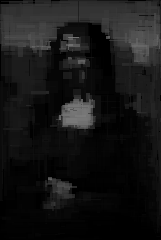
\includegraphics[width=\textwidth]{images/mona/dependence/1000_500.png}
         \caption{1000 pokoleń, 500 osobników w pokoleniu}
    \end{subfigure}
    \begin{subfigure}[b]{0.3\textwidth}
        \centering
        \label{fig:dependence_500_1000}
         
\includegraphics[width=\textwidth]{images/mona/dependence/500_1000.png}
         \caption{500 pokoleń, 1000 osobników w pokoleniu}
    \end{subfigure}
    \caption{Wyniki prezentujące zależność pomiędzy liczbą pokoleń algorytmu a licznością pokolenia}
    \label{fig:dependence_rep}
\end{figure}

\subsection{Obserwacje}
Można zauważyć, że czas działania dla każdej z konfiguracji parametrów jest w przybliżeniu taki sam (ponad 4 minuty). Na grafice \ref{fig:dependence_rep} widać wyraźnie, że wraz ze wzrostem liczby pokoleń i jednoczesnym zmniejszeniem liczby osobników w pokoleniu znacznie pogorszyła się, pod względem wizualnym, jakość uzyskanego rozwiązania. Uzyskany rezultat jest bardzo odległy od oczekiwanego - sylwetka postaci przedstawionej na obrazie oryginalnym jest prawie całkowicie niewidoczna.  Najlepsze wyniki uzyskano dla przypadku, gdy ograniczono liczbę iteracji algorytmu (do 1000-500) a zwiększono liczbę osobników tworzących dane pokolenie - na tych obrazach wyraźnie można wyróżnić prezentowaną na obrazie postać oraz zarysy elementów tła.

\subsection{Wnioski}
Na podstawie przeprowadzonych obserwacji można stwierdzić, że w przypadku, gdy wymagane jest narzucenie ograniczenia czasowego na program, lepszym wyborem będzie zwiększenie liczby osobników w pokoleniu kosztem zmniejszenia liczby iteracji programu. 

\section{Podsumowanie}
W niniejszym rozdziale dotyczącym analizy uzyskanych wyników przedstawiono wyniki testów, które miały zbadać wpływ możliwych do ustawiania przez użytkownika parametrów, które, potencjalnie, mogą mieć największy wpływ na jakość uzyskiwanych rozwiązań. Po analizie przedstawionych obserwacji oraz wniosków można zauważyć, że algorytm lepiej radzi sobie z obrazami, zawierającymi mniej szczegółów oraz w jednolitej skali kolorystycznej - skali szarości. Obserwator może również stwierdzić, że algorytmowi trudniej odwzorować obszary ciemniejsze, a dokładniejsze odwzorowanie pierwowzoru otrzymuje się w przypadku obrazów jaśniejszych. W kontekście możliwych rozszerzeń pracy należałoby przebadać jakość uzyskiwanych rozwiązań dla, na przykład zdjęć zrobionych w dobrych warunkach oświetleniowych, obrazów namalowanych w jasnych kolorach lub zdjęć prześwietlonych.

Autor chce zauważyć, że jest to jedynie niewielka część różnych zestawień konfiguracji algorytmu, które mogłyby zostać zbadane. Zdecydował się on na zaprezentowanie jedynie tych, które według jego uznania pokazywały w najlepszy sposób zarówno mocne, jak i słabe strony opisywanego algorytmu. Ze względu małej ilości czasu autorowi nie udało się przeprowadzić wszystkich zamierzonych testów. Sugerowane ścieżki testowania i oceny generowanych rozwiązań to:
\begin{itemize}
    \item zbadanie subiektywnej oceny osób trzecich w postaci ankiety i późniejsza jej analiza,
    \item zbadanie innych metryk oceny jakości rozwiązań (funkcja celu),
    \item zbadanie jak algorytm poradzi sobie z obrazami w dużych rozdzielczościach, na przykład \textit{FullHD},
    \item zbadanie dokładnego profilowania pamięci podczas działania programu, na przykład za pomocą narzędzia \texttt{Valgrind}.
\end{itemize}

    \cleardoublepage
	
	\chapter{Podsumowanie}
\thispagestyle{chapterBeginStyle}

W podsumowaniu zostaną zawarte wnioski wyciągnięte z pracy (oraz procesu jej tworzenia).
	\cleardoublepage
	
	
	%%%%%%%%%%%%%%%%%%%%%%%%%%%%%%%%%%%%%%%%%%%%%%%%%%%%%%%%%%%%%%%%%%%%%%%%%%%%%%
	%%%%%%%%%%%%%%%%%%%%%%%%%%%%%%% BIBLIOGRAFIA %%%%%%%%%%%%%%%%%%%%%%%%%%%%%%%%%
	%%%%%%%%%%%%%%%%%%%%%%%%%%%%%%%%%%%%%%%%%%%%%%%%%%%%%%%%%%%%%%%%%%%%%%%%%%%%%%

	\pagestyle{bibliographyStyle}
	\bibliographystyle{plabbrv}
	\bibliography{literatura}
	\thispagestyle{chapterBeginStyle}
        \addcontentsline{toc}{chapter}{Bibliografia}

	\cleardoublepage
	
	%%%%%%%%%%%%%%%%%%%%%%%%%%%%%%%%%%%%%%%%%%%%%%%%%%%%%%%%%%%%%%%%%%%%%%%%%%%%%%
	%%%%%%%%%%%%%%%%%%%%%%%%%%%%%%%%% DODATKI %%%%%%%%%%%%%%%%%%%%%%%%%%%%%%%%%%%%
	%%%%%%%%%%%%%%%%%%%%%%%%%%%%%%%%%%%%%%%%%%%%%%%%%%%%%%%%%%%%%%%%%%%%%%%%%%%%%%
	
	\appendix
	\pagestyle{appendixStyle}
	
	\chapter{Zawartość płyty CD}
\thispagestyle{chapterBeginStyle}
\label{plytaCD}

W tym rozdziale należy krótko omówić zawartość dołączonej płyty CD.


	\cleardoublepage

\end{document}

